% The paper's records: the blocks cut from main.tex at 48 pages (the owner's
% words of 2026-09-23, "48 pages" and "there is only one paper"), kept verbatim
% from the same source by cut30/assemble.py (cut30/records.py); edit the parts,
% not this file. This is a source file of the archive, cited from the paper as
% \cite{records}; it is not a document and is not compiled on its own: its
% references (\ref, \eqref, \cite) are the paper's.
\section{The confrontation register, the full record}\label{app:register}

{\scriptsize\setlength{\tabcolsep}{3pt}
\begin{longtable}{L{0.3in}L{2.0in}L{1.5in}L{2.2in}}
\caption{\label{tab:nature}The confrontation register, the full record, every row \cite{nature}, with the law's own number and a status of three values, agrees, disagrees, not predicted (its missing piece and kind), defined in Section~\ref{sec:comparison}; the kinds in every cell: DETECTOR a count of clicks, the only measurement; GAMEBOARD a number of the board's state, a diagnostic; COMPUTATION the algebra's number, no run; the model's numbers are ideal, at the registered grain, not a prediction for a given instrument. The one count, repeated in the abstract and in Section~\ref{sec:physics}: the paper's list of Table~\ref{tab:list} is closed in the algebra before any run, every pinned reading a blank until its run is read and merged, and none is read yet on the engine as it stands; the old count of the engine before 2026-09-23 is history \cite{records}; the hypotheses beside rows 6, 13 and 14 change no verdict of the law (the PASS rows replicated \cite{replications}). Each reading's kind is named: DETECTOR (a click), GAMEBOARD (the host's view, a diagnostic) or COMPUTATION (the algebra's); the criteria row by row, with the re-runs at head, are \cite{criteria}.}\\
\toprule
Row & Observable and nature's value & The law's reading, by kind & Status \\
\midrule
\endfirsthead
\toprule
Row & Observable and nature's value & The law's reading, by kind & Status \\
\midrule
\endhead
\bottomrule
\endlastfoot
1a & The CHSH sum of a pair: $2.42 \pm 0.20$ \cite{hensen2015}; the quantum bound $2.828$ & $S = 2.75$ at $\Nphi = 64$, series L (DETECTOR; replayed at head by the test suite) & agrees: $S = 2.75$ at $\Nphi = 64$ (DETECTOR), $1.65$ standard errors above the measured, $0.078$ below the quantum bound; the pair by the click, Section~\ref{sec:click} \cite[section 10]{clickframe} \\
1b & The same, the phase-form window & $S = 2$ exactly (DETECTOR, the counters' clicks) & a control, not counted: $S = 2$ exactly (DETECTOR), the local bound, $2.1$ standard errors below the measured; Bell's bound is a theorem of every local read-out and the phase-form window is one, the law's answer to nature being row 1a \\
1c & No signalling in the order: nature $0$ on the second party's serial correlation at lag $1$ under the first party's settings (the outcome order of a pair random, carrying no setting of the other party; the marginals' independence holds in nature and in the law alike) & $15/16$ under a constant $a = 0$ and $-1/16$ under the period-$3$ cycle $a = 0, 21, 42$, cyclic over $192$ births on the registered pair world at $\Nphi = 64$ (DETECTOR, the run of 2026-09-22 \cite{orderchannel}); the marginals $96/96$ under both (DETECTOR); the algebra's $15/16$ and $-1/16$ met at $16$ of $16$ checks; the cycle $\Nphi/2, 0, 0$ of Section~\ref{sec:bell}, $-5/16$, a computation the register's keys cannot declare & disagrees: $15/16$ and $-1/16$ (DETECTOR) against nature's $0$; the law's determinism, the wheel a counter, shows in the order and not in the counts \\
2a & Two-slit visibility of one quantum at a time: $0.98$, the register's source \cite{grangier1986} a Mach-Zehnder reading and not a two-slit one; a two-slit source, a Fresnel biprism's central fringe at $0.94$ as reported \cite{jacques2005}, its figure to be verified against the source; the ideal $1$; the criterion the clicks' visibility $(I_{\max} - I_{\min})/(I_{\max} + I_{\min})$, no apparatus model & $0.966$ in the clicks of \texttt{slits\_huygens} (the birth wheel, $4096$ births; L2b; DETECTOR), the pin derived for this world's fan by the register's own algebra $0.9659$ (COMPUTATION) and met bit for bit by the re-run at head, $0$ of $121$ pixels differing; the record's weights read the same under the exact phase (the $0.954$ of the built-phase pin of 2026-09-20 is history) & NOT COMPARED until the two-slit source is verified; the law's number $0.966$ in the clicks (DETECTOR) a prediction under every fan (the grain's share at most $12$ percent of the shortfall, $0.004$ of $0.034$, the kind audit \cite[section 3]{kindaudit}, COMPUTATION); a bound met against the biprism's $0.94$ at the abstract's level \cite{jacques2005}; against the Mach-Zehnder's $0.98$ another geometry \\
2b & Mach-Zehnder visibility: $0.98$ \cite{grangier1986}; the criterion the visibility $(b - d)/(b + d)$ of the bright and dark ports' offers of \texttt{mz\_equal}, no apparatus model & the offers $1681/1682$ and $1/1682$ (GAMEBOARD, the record's ledger); the clicks $64/0$ over $64$ births (DETECTOR; replayed at head by the tests) & agrees, a bound met and not a quantitative agreement: the clicks' visibility $1.000$ ($64/0$, DETECTOR) above the apparatus-limited $0.98$; the offers' $0.9988$ a GAMEBOARD diagnostic of the apparatus layer \\
2c & The power of the click's form: the Sorkin parameter $\kappa_{\mathrm S} = 0.0064 \pm 0.0119$ \cite{sinha2010} & the power's window $[1.917, 2.012)$ from the click cells (DETECTOR), a read-back of the built click (COMPUTATION) & NOT COMPARED ($\kappa_{\mathrm S}$ not computed): the window an implementation gate, no evidence about nature; no three-opening world is registered \\
3 & The deceleration parameter $q_0 = -0.53 \pm 0.01$ \cite{planck2018,riess1998,perlmutter1999} & $-0.108$ coasting (series G2, the pointer's $z$: read at head in the detector's own clock, its count of self-creations under the age wall ($r = 1.0000$, no crowd at the detector; \cite{criteria}, the re-run of 2026-09-22), equal to the host's interval to the integer, DETECTOR; the registered run's time base was the host's interval \cite[record 768]{log}, superseded; a two-way light clock at the detector, not read, reads the same count in no crowd (series X)); $-0.104$ at head (\cite[record 408]{log}; the re-run at head, the pin met, DETECTOR), the reading's own grain $0.004$ between engines and $0.03$ between windows & not predicted, kinds (1) and (2): the law's number $-0.108$ coasting (DETECTOR, the detector's own clock), the coasting ideal $q = 0$ within the reading's grain, $0.42$ from nature's value; the crowd's history is missing, no term carries $q$ toward $-0.5$ and the law's own crowd gives the wrong sign; nature's $-0.53 \pm 0.01$ is a fitted parameter of the diagram \\
4a & The muon's lifetime in flight over its lifetime at rest: $\gamma = 29.33$ at the storage ring, the dilation confirmed as $\gamma$ to a fractional error of about $2 \times 10^{-3}$ \cite{bailey1977} & the \texttt{become} at the count $64$ at every speed (a body's own record, DETECTOR; its interval GAMEBOARD), the products' face clicks (DETECTOR): the ratio $1$; under covariant-readings-v1 within its domain, the products' clicks $367$ and $344$, the ratios $70/64$ and $124/64$ against $\gamma = 1.1074$ and $1.9558$ (DETECTOR) \cite{run4ab} & not predicted, kind (1): no moving thing's clock rate, $r = 1$; the law's number $1$ against $29.33$; beside it, as a declared hypothesis, $\gamma$'s form within the domain $\gamma \le 2$ \cite{run4ab}, nature's $29.33$ outside the domain under either drive, a factor $14.8$ short at the cap \\
4b & A moving lamp's redshift with the clock's factor \cite{botermann2014} & $z = 0.2636$ at $\beta = v/c = 0.2674$ (series G2: read at head in the detector's own clock, its count of self-creations under the age wall ($r = 1.0000$, no crowd at the detector; \cite{criteria}, the re-run of 2026-09-22), equal to the host's interval to the integer, DETECTOR; the registered run's time base was the host's interval \cite[record 768]{log}, superseded; a two-way light clock at the detector, not read, reads the same count in no crowd (series X)); $0.2647$ at head (the re-run, the pin met, DETECTOR) & not predicted, kind (1): the law's number $0.2647$ (DETECTOR, the detector's own clock) against $0.315$, $17$ grains below, $1 + z = 1 + v$ with no moving clock's rate ($r = 1$); beside it, under covariant-readings-v1 as a declared hypothesis, $0.3674$ for $0.369 \pm 0.003$, read at a click over the detector's own count, $0.3674$ in $[0.366, 0.372]$ \cite{run4ab}; the two one-way factors apart by $1 - v^2$ under the law and at $1$ within $0.4$ percent under the key, read on the $k$-ladder \cite{run4ab} \\
5a & The anisotropy of $c$ by direction, below $10^{-18}$ \cite{nagel2015} & the flight table's pace $0.5774$ to $0.5818$ at $N_l = 64$ (COMPUTATION; series Q's $290$ of $290$ clicks within it at finite ages, DETECTOR, Appendix~\ref{app:reproduction}) & agrees, a bound met: the pace $0.5774$ to $0.5818$ by direction (COMPUTATION; series Q's $290$ of $290$ clicks within it, DETECTOR), isotropic within $1/T_D$; a bound on $N_l$ of order $5.8 \times 10^{17}$ for nature's $10^{-18}$ \\
5b & The anisotropy of $c$ between a laboratory's two arms when the laboratory moves: the null at the Earth's $\beta = 10^{-4}$ \cite{michelson1887} & the round trips $\gamma^2$ along the motion and $\gamma$ across on the flight table, $1.375$ and $1.140$ at $\beta = 0.4297$ (COMPUTATION, a pin; the pair in motion not run) & not predicted, kind (1): nothing contracts, the bond a whole Link and a contraction a root of the state at run time; the pin's arms differ by $\beta^2/2 = 5 \times 10^{-9}$ at $\beta = 10^{-4}$, eight to nine orders above the bound \\
6 & Bohr's line ratio $\nu(\mathrm{H}\beta)/\nu(\mathrm{H}\alpha)$ of the Balmer series: $1.3500$, $656.279$ over $486.135$ nm \cite{nist}, Balmer's $27/20$ exactly & by algebra first, on the law's integers (COMPUTATION \cite{atomalgebra}): a closed loop is an integer congruence of the action row, $\Delta A_a = 0 \bmod h$ on each axis with the quotients summing to $jN$; two closing radii stand as the square of two counts a detector reads, $a_j/a_i = (j/i)^2$ in the shell mean, checked by $T_j/T_i = (j/i)^3$, no root, no float; from a closed circle one click reaches only the loops with $2i^2 \ge j^2$ and a release of content unbinds, so no line of Balmer's is one click of the law: NEEDS A NEW RULE. The law as built: the electron escapes at $3407$ intervals (series H's world, DETECTOR; the cause the half-Link lag \cite{atomcause}). Under the key \texttt{centred\_step} (a declared start of the drive, off by default; Section~\ref{sec:click}): the loop stays, no escape face click in $7500$ intervals, $23$ quarter crossings (C1 PASS, DETECTOR), tightening from $12$ to $7$ Links at two crossings over five turns, the period falling from $1431$ to $1040$ (C2, C3 FAIL as declared, DETECTOR; the run of 2026-09-22 \cite{atomcentred}); no line read & disagrees: the loop opens at $3407$ intervals (DETECTOR) and no line is read, against Balmer's $27/20$; under the key C1 PASS, C2 and C3 FAIL, no pin moved; no rule of the six quantises a body's loop, so the lines are computable by no run of the law as built and $27/20$ waits on a rule under its own identity; the ladder $a_j/a_i = (j/i)^2$, $E_j \propto 1/j^2$ and Balmer's $27/20$ conjectured from the algebra in the shell mean's limit, not read on the board; a lattice able to hold the scale (the orbit's radius sixty thousand times the nucleus's) is not run (Section~\ref{sec:discussion} (viii)) \\
7a & The deuteron's binding fraction $0.1185$ percent \cite{ame2020} & the bond's two border clicks and the mass read $3673$ (DETECTOR) against the declared $3677$, $4$ units, $0.109$ percent (series N); the books' escaped $4$ (GAMEBOARD, a diagnostic) the check; the same at head, every pin met & not predicted: the give per nucleon a declared input read back \cite[record 106]{log}; the escaped $4$ of $3677$ (DETECTOR) brackets nature's $4.35$ between the whole gives $4$ and $5$; the missing piece a rule that derives the binding; the law's number the mass read $3673$ against the declared $3677$ (DETECTOR), $0.109$ percent \\
7b & The alpha's binding over the deuteron's, $12.72$ \cite{ame2020} & $2.0$ (series N, the border's four clicks against two, DETECTOR; the same at head) & disagrees: $2.0$ (DETECTOR) against $12.72$, a factor $6.4$; the give once per body \\
8a & The neutron's decay curve, exponential, width over median $3.17$ \cite{gonzalez2021} & a step: every neutron at its key on its own clock, the width $0$ (DETECTOR, the $64$ clicks of content $3$); the width over the median in the lattice's clock $0.036$ in the registered run and $0.08$ to $0.13$ at head at the cap $1024$ (GAMEBOARD, the lattice's clock, counted in no criterion; against nature's $3.17$ these widths would read a factor $88$ in the registered run and $25$ to $40$ at head, numbers of the diagnostic that stand in no verdict) & disagrees: a step, the width $0$ (DETECTOR) against nature's $3.17$, the step the law's own prediction; a width would need a decay fired by a met row of a declared bath (\cite[section 1.8]{failrows}), none of the three pieces; the width in the lattice's clock a diagnostic beside it; the registered J1 run predates the one flight wall, under which the weak register's become blocks move (\cite[records 931 to 933]{log}), J1's redeclaration in the weak field after the paper \\
8b & The neutrino's passage through a second detector, about $1$ & $16$ of $1024$ with $0$ behind (series J2, a window; DETECTOR; the same at head, the pin met bit for bit) & disagrees: $16$ of $1024$ and $0$ behind (DETECTOR, series J2) against nature's about $1$; under the declaration massive-rows-v1 with the $\nu$ quantum $1$ the readers read $0$ and $0$ and the reader at the Node of a whole turn the whole beam, $1013$ of $1013$, the far detector $0$, by the law's design of the path phase, the beat $h/p = 4.65$ Links read at a click for the first time \cite{run8bc}; beside it, with a re-emitter declared between the source and the readers, an arrangement of the law and not nature's, the second reader's rate over the first's is $1.000$ exactly ($16$ of $1024$ and $16$ of $1007$, the far detector $683$ of $705$, DETECTOR) \cite{run8bc}, not a pass against nature \\
8c & The heaviest neutrino mass state over the electron's mass: at least $9.8 \times 10^{-8}$ \cite{pdg2024,katrin2022} & the \texttt{nu} family with no content, an input & not predicted, kind (2): the family's content is a declared input, and nature's number a bound; the law's number $0$, the \texttt{nu} family with no content, refuted as an input by the observed splittings; under massive-rows-v1 the quantum $1$ is the input no longer $0$, a computation and no click, the electron's declared content then at least $1.02 \times 10^7$ units (COMPUTATION) \cite{run8bc} \\
9 & Malus's law at $45$ degrees, $1/2$ & $128$ of $256$ exactly; $219$ of $256$ at $22.5$ degrees (A12; DETECTOR, replayed at head by the tests) & agrees: $128$ of $256$ exactly at $45$ degrees (DETECTOR), exact at $45$ and $90$; $0.8555$ against $\cos^2 = 0.8536$ at $22.5$, within the tables' grain \\
10 & The single-opening spread $w\,\Delta(\sin\theta)/\lambda$: $0.886$, the full width at half maximum of the single-slit pattern \cite{nairz2002} & the register's entry A10: $1.08$ at $w = 27$ with $\lambda = 4.619$ Links (the crowd form, kept as history); the record form's re-run did not complete & NOT YET under the one click, as it is: the last registered $1.08$ against $0.886$, $22$ percent above; the smaller widths unread \\
11a & The deceleration parameter read from the brightness of a far lamp: $-0.53 \pm 0.01$ (row 3's sources) & a derivation's pin, $q_{\mathrm{eff}} = +1$: the click count falls as $1/(1 + z)$ and the content per click stays the birth's, one factor where nature's flux has two (COMPUTATION; the run not made) & not predicted, kinds (1) and (3): no term of the crowd's history, and no click definition of a brightness yet; the pin $+1$ against $-0.53$ \\
11b & The stretch of a far lamp's stream over $1 + z$: the exponent $b = 0.97 \pm 0.10$ of $(1 + z)^b$ \cite{blondin2008} & the same pin: $400$ rows released over $400$ intervals arrive over $1452$ at $300$ Links, the factor $3.639$ against $e^{Hd/c_0} = 3.629$, $b = 1$ (COMPUTATION; the run not made) & PASS by its pin, as it is: $b = 1$ within $0.97 \pm 0.10$; pinned, the run not made, a pin needing a hypothesis not built \\
11c & Tolman's test, the surface brightness of a resolved source at $z$: $(1 + z)^{-4}$, measured as $(1 + z)^{-n}$ with $n$ between $2.3$ and $3.1$ before correction \cite{lubin2001} & the same pin: the board's Nodes and the fan's lines fixed under the wall, a ruler of $l$ Nodes at $d$ subtends $l/d$, the flux one power of $1 + z$, $n = 1$ (COMPUTATION; the run not made) & not predicted, kinds (1) and (2): an angular size growing with the redshift is a board whose Links stretch, no verb on the state; nature's exponent a fitted value; the pin $n = 1$ against $4$, three powers of $1 + z$ at most \\
12 & The clock's field at two distances at the same push: the potential's form, $2.00$ (the GPS term $45.7$ microseconds per day \cite{ashby2003}; \cite{pound1960,delva2018}) & series T: the form measured at a detector at two Nodes (the ratio of the two records' rates over the same intervals, in which the interval cancels (DETECTOR)), the age clock $1.907$ (the lines' pin $1.909 \pm 0.05$), the presence clock $1.000$ & read under the law before the generic entry of 2026-09-22 \cite{genericentry}; not readable under the law as it stands; the four worlds are being redeclared in the weak field (the pair $[1, 16384]$, the crowd's age moment at most $1024$ per Node on the light's path) and re-read, the new numbers to replace these; HISTORY, not a pass: under the age word (P9) as the form at two Nodes the lattice pin $1.909 \pm 0.05$ is met (DETECTOR, a gate on the code, the law before the entry), the lattice's dwelling ages $5, 6$ and $10, 11$ pinning $1.909$ for the continuum's $2.00$; against nature the reading $1.907$ is $4.6$ percent off with no uncertainty stated on either side, so the caption's PASS criterion is met nowhere, PENDING the weak-field re-read; FAIL under the presence word \\
13 & The bending of light beside a mass, the full deflection over the time part's alone, $1 + \gamma = 2$ at the Sun's limb, $1.75$ arcseconds against the time part's $0.87$ \cite{dyson1920} & the law as built at head, on a coupled world: the centroid shift $-1.993$ pixel and the delay $2.95$ intervals at $\gamma_{\mathrm{PPN}} = 0$ (DETECTOR, \texttt{optical/mass\_g0} against \texttt{control\_g0} at head), the pin $-1.93 \pm 0.5$ met, the audit's re-run \cite{disagrees}; half of the declared $\gamma_{\mathrm{PPN}} = 1$ world's $-3.989$: the time part alone, a factor $2$ against nature's $1 + \gamma = 2$ under the register's conversion (COMPUTATION on two DETECTOR shifts through the declared weight rule; record 1216). Series K's $0.000$ pixel and $0.00$ interval (three worlds, DETECTOR) are the reading of worlds that declare suspension $0$, at which a row's coupling to the crowd is zero by declaration: history, not the law's number on a coupled world. By algebra first, on the law's integers (COMPUTATION): the walk of a light row past a held mass under the key \texttt{optical}, read at a ring of Nodes at the impact distance $b$, recovers the $M/b$ form with $C_{\mathrm{ring}} = \alpha b c^2/(GM) = 5.12$ at $b = 6$ ($5.44$, $5.86$ at $b = 3$, $8$), not $4$ within the ring's grain, the factor left the fan's $F_{L1} = 1.421$ of the flow \cite{stepalgebra}; under the one constant (flow-link-v1, the flow counted per Euclidean Link of its line) $C_{\mathrm{ring}} = 3.65$, $3.82$, $3.92$ at $b = 6$, $3$, $8$ against $4$, that is $2c_f$ within the finite path's $L/\sqrt{L^2 + b^2}$ ($0.974$ at $b = 6$) and the shells' $0.990$, one to three grains, $4 = 2(1 + \gamma)$ with $\gamma$ an input \cite{flowalgebra}. The run of 2026-09-22 on the split ladder (the wall's square reached without the root; the first run's deciding ring had been refused by the working bound) \cite{ringrun}: Under flow-link-v1 (the key \texttt{flow\_link}, off by default) the six ring worlds read their mean radial shifts at the algebra's numbers ($b = 6$, $\gamma = 1$, the deciding pin: $0.731$ Links against $0.731 \pm 0.025$; every arrival Node the map's, $168$ of $168$; DETECTOR), and the constant through the stated lever-arm factor, $C_{\mathrm{ring}} = 3.655$, $3.819$, $3.918$ at $b = 6$, $3$, $8$ and $\gamma = 1$ (COMPUTATION), is the algebra's own walk to $0.01$ and $2.40$, $1.07$, $1.40$ grains from the continuum's $2c_f \times 0.990 \times L/\sqrt{L^2 + b^2}$, outside the one-grain pin: the engine walks the rule as the algebra walks it, and the bending's $4$ does not close within the grain ($3.655$, $3.819$, $3.918$ bare against $4$); $c_f = 2$ is an input, $nS = d$ a declaration, $4$ on the comparison side; nothing here is compared with nature. & disagrees: the law as built $-1.993$ pixel at $\gamma_{\mathrm{PPN}} = 0$ (DETECTOR), half of nature's by the time part alone, a factor $2$ against $1 + \gamma = 2$, $1.75$ arcseconds; series K's $0.000$ history; beside it, under the declaration $\gamma_{\mathrm{PPN}} = 1$ (the weight rule, stated once in the limitations paragraph), the ring's rule read inside its pins, the deciding ring $0.731$ against $0.731 \pm 0.025$ (DETECTOR), the coefficient $2(1 + \gamma_{\mathrm{PPN}})$ a declared input equal to nature's, read within the fan's comb ($3.65$, $3.82$, $3.92$ against $4$, two to nine percent) and never within the grain, a declared input and not a prediction; the ring's shift and the ratio read the declared $\gamma_{\mathrm{PPN}}$ back (DETECTOR readings of a declared input); the coefficient on the one constant stays conjectured from the algebra \\
14 & Newton after a detector: the ratio of the periods of two closed loops at $r = 24$ and $12$ under the $1/r$ push on the plane, $2.00$ (the form's scale symmetry; nature's inverse square in space $2^{3/2}$); the register's bracket $2.00 \pm 0.18$; the run's loops never closed, so its ratio is not compared with nature & by formula first (COMPUTATION \cite{flowalgebra}): under the one constant every push is divided by the plane fan's mean of $S_1/|\mathbf D|$, $F_{\mathrm{plane}} = 1.2871$, so the circular balance solves to the whole $n = 8$ and the periods $T = 2\pi r(S + n)/n$ move from $343$, $687$ to $384$, $768$ ($377$, $754$ at the whole $8$), the ratio $2.00$ unchanged, the factor a constant of the line cancelling in it. The run of 2026-09-22 under the key \texttt{flow\_link}, series D3's four worlds, the pins by the generator before any run \cite{newtonrun}: the controls inside (every click at $x = c_x + r$; the escape tick $305$ in $299$ to $311$; DETECTOR); the probes escaped, \texttt{r12\_flow} through the face $+y$ at the tick $1208$ and \texttt{r24\_flow} through the face $-x$ at $2452$ (face clicks, DETECTOR, read from the registered events by the diagnosis \cite{newtondiagnosis}; the run's first record had read none), so no loop closed, and the readings called periods are the means of the recurrences of $x$ before the escape, two and three unequal spacings, outside: $T(12) = 588.7$ against $343.1$ to $410.9$, $T(24) = 987.3$ against $686.1$ to $821.8$, $\omega^2 = 7.775 \times 10^{-5}$ (the angular rate squared) and $3.112 \times 10^{-5}$ against $2.338$ to $3.354 \times 10^{-4}$ and $5.845$ to $8.386 \times 10^{-5}$, the amplitudes $32.5$ and $45$ against $11$ to $14$ and $23$ to $26$ (DETECTOR); the ratio $T(24)/T(12) = 1.677$ against $1.82$ to $2.18$ (COMPUTATION from two means of unclosed loops' spacings, not a reading of the force's exponent; the two loops are not similar figures, their mean radii $24.3$ and $37.6$, CONVERSION, so the $1/r$ form's scale symmetry is not tested by them); $4$ inside, $7$ outside, none moved, $0$ record checks failed; the registered D3 row at $n = 9$ ($7$ inside, $9$ outside; Section~\ref{sec:forces}'s $1.997$) stays as history beside it & not yet read against nature: the law's number $1.677$ under the one constant and $1.512$ under the line drive (COMPUTATION on the host's tick of unclosed loops; the register's $2.00 \pm 0.18$ a host-tick period; the D3 probes left a confining push and no loop closed, the face clicks DETECTOR); the law as built $1.997$ in $[1.82, 2.18]$ on the plane's $1/r$ form (Section~\ref{sec:forces}), the inverse square in space NOT MADE; read under the declaration of the weight rule (the limitations paragraph). The run of 2026-09-23 \cite{run14}: the click algebra's rung confirmed by the control ($979$ then $980$, DETECTOR); the conditional pins, the law's shell-mean form on an input no click read, FAIL on this fan by the comb ($2.5$ to $4$ times, DETECTOR against a conditional pin); nature's period not compared \\
\end{longtable}}



\section{The check of the roads}\label{app:families}  {\scriptsize\setlength{\tabcolsep}{3pt} \begin{longtable}{L{1.5in}L{1.75in}L{1.5in}L{1.4in}} \caption{\label{tab:roads}The check of the roads (record 817): one row per formula the paper arrives at, the inputs its chain used, the file and line where the chain starts (the click frame on \texttt{main} at 70e9781a \cite{clickframe}; Einstein Outside at e8432e6c \cite{einsteinoutside}, whose section III is the same check in the source) and the word. No row lists Einstein's or Lorentz's formula among its inputs; ``derived'' stands in no row.}\\ \toprule The formula arrived at & The inputs its chain used & Where the chain starts & The word \\ \midrule \endfirsthead \toprule The formula & The inputs & Where & The word \\ \midrule \endhead \bottomrule \endlastfoot $W = E_0'^2 + 3\,\mathbf p\cdot\mathbf p$ to second order & (A1), (A2); the walk's invariant $\cos\omega = \cos m\cos\kappa$; the Planck map on \texttt{main}; the unit $E' = E/c^2$ & the click frame, section 7 & shown to second order (the conversion's identity); declared for the rows' dynamics (record 270) \\ the boost, Lorentz's form & (A1); two legs at one Node per interval; $k_{AB} = k_{BA}$ & the click frame, section 2 (b) :278--297; section 0 :84--132 (the group up to scale) & follows; Lorentz's form recovered, the scale $r$ free; (A2) fixes $r$ at $\sqrt{1 - v^2}$ \\  $1/\gamma$, the rate $r$ & Theorems 1, 2; $r$ read from two factors & Einstein Outside, II.1 :647 & follows in $r$; $\sqrt{1 - v^2}$ recovered under the line, shown to second order under (A2), declared under the identity, $1$ on the law \\  $E^2 = E_0^2 + c^2p^2$ & $E = E_0/r$, $p = Ev$, the line of II.1; the frame's section 7 for $W$ & Einstein Outside, II.6 :887 & follows as the line; $W$ shown to second order; exact by declaration under the identity; $E_0 = mc^2$ a declared unit \\ the Outside step, place apart and count apart of a detector, Einstein's step its most general form & (A1), (A3), the Inside step, Theorems 1, 2 & Einstein Outside, section 3 (a) :481 (Einstein's form named at :497 as the comparison) & follows; Einstein's form recovered where $r$ is supplied, never an input \\  Newton's step as the limit & Theorem 4, the shell mean, $v \ll c$ & Einstein Outside, section 3 (c) :554 & recovered (the limit) \\ \end{longtable}}  



\section{Reproduction: the runs, the fingerprints and the seven confirmations}\label{rec:reproduction}

The code, the worlds with their expectation files written before the runs, the check scripts with their outputs, the runs' summary and the figure scripts are archived \cite{zenodo}; the register carries every run's world, duration and source fingerprint, and NUMBERS.md beside the manuscript maps each number of this paper to its source \cite{checks}; the criterion of every row of Table~\ref{tab:nature}, what is measured, its kind, what would refute it and the re-run at head, is \cite{criteria}. The register's consolidation (its head \texttt{b12dd253} on the branch \texttt{register-paper-sources}, pending merge; the merge commit replaces it) keeps every world this paper cites, and the worlds it removes are cited by no row of this paper; NUMBERS.md marks the rows whose worlds the paper no longer cites. The interpreter is Python 3.14, no floating point in any physical module, the runs seconds each. To run a registered world from the archive: \texttt{python -m pip install -e .} and then \texttt{python -m event\_universe --init} \texttt{examples/events/amplitude/bell\_0\_24.json} \texttt{--output artifacts/bell\_0\_24}; the worlds of this paper are under \texttt{examples/events/amplitude/}, the pair \texttt{bell\_*.json}, the two slits \texttt{slits\_huygens.json}, the Mach-Zehnder \texttt{mz\_equal.json}, \texttt{mz\_half.json} and \texttt{mz\_quarter.json}; a run writes its metadata and its events beside the output, and the check scripts read them. The runs' fingerprints: the register's \texttt{ff5c382d672f} (series L), L7 \texttt{4bf55a62e6fd}, S \texttt{24e0c1ba}, T \texttt{afb533a}. The figures' runs carry the fingerprint \texttt{731d0f56c9f9} (\texttt{figures/summary.json} \cite{checks}). 

\paragraph{The seven confirmations.} {\footnotesize Each a run's clicks against the formula shown Inside, the rows in Tables~\ref{tab:nature} and~\ref{tab:families}: the pace, series Q, $290$ of $290$ primitive directions ($|a| + |b| + |c| \le 6$) at the derived interval, Node and face, $0.5718$ to $0.5893$ at finite ages; the click's power, series L, the $(3, 4)$ split $63/1$, $31/1$, $125/3$ at $\Nphi = 64$, $32$, $128$, the far pair's cells $27, 5, 5, 27$; Mach-Zehnder, $64/0$ equal arms, $0/64$ at a half turn, $32/32$ at a quarter, over $64$ births; the marginals, $32/64$ per party in every bin at $\Nphi = 64$; GHZ, the four allowed triples $16$ each, the products $+1$ and $-1$, the others $0$; Malus (A12), $128$, $0$ and $219$ of $256$ at $45$, $90$ and $22.5$ degrees; light beside a mass, series K, three worlds, the deflection $0.000$ pixel, the delay $0.00$ interval \cite{register,replications}.} 

\section{Auxiliary proofs}\label{app:proofs}

\paragraph{Proof of Theorem~\ref{th:group}.} A map of the six Ports that keeps opposite Ports opposite is a signed permutation of the three axes, $3!\,2^3 = 48$ of them, the hyperoctahedral group $B_3$; the determinant is a homomorphism onto $\{+1, -1\}$, so its kernel, the group of order $24$, has index $2$ and acts faithfully on the cube's four body diagonals, so it is the symmetric group $S_4$ on them; a pseudoscalar column goes to $\det(g)$ times itself by definition. 

\paragraph{Proof of Theorem~\ref{th:isometry}.} $\sum_i (wa_i)^2/(\mathtt m A) = w^2/\mathtt m$. The conjugate transpose maps the outputs $(wa_i, \mathtt m A, p + t_i)$ to $(Aw, A^2 \mathtt m, p) \sim (w, \mathtt m, p)$; for two inputs at one splitter the cross terms carry phases differing by $\Nphi/2$ and cancel in the normal form, which the check with the pairs $(20, 21)$, $(3, 4, 5)$ and $(119, 120, 169)$ confirms integer by integer \cite{design}, and the engine's merge reproduces on its own rows \cite{beamlaw}. That cancellation is the joint condition $B^{\mathsf H} B = 2I$ of the balanced splitter's table $\begin{pmatrix} 1 & x^{\Nphi/4} \\ x^{\Nphi/4} & 1 \end{pmatrix}$, and the condition is needed: two inputs declared $(1, 1)$ with the turns $(0, 0)$ onto the same two outputs have the table $\begin{pmatrix} 1 & 1 \\ 1 & 1 \end{pmatrix}$, which sends $(1, -1)$ to $0$ and merges the inputs $(1, 3)$ and $(2, 2)$ to the same $(4, 4)$ (the exact witness of the independent read of 2026-09-22); each column keeps its own $w^2/\mathtt m$ there and the joint map does not, and Rule S as a generic rule admits such a table; no world of this paper declares one. For $U_s$ the diagonal of $U_s^{\mathsf T}U_s$ is $C'^2 + S'^2$ and the off-diagonal $C'S' - S'C' = 0$ in integers.

\paragraph{Proof of Theorem~\ref{th:bijection}.} $F$ maps a basis element of $Q$ to a basis element, the Node moved by an offset that is a function of $D$ and of the age, the history's, so with the history fixed it is injective on the basis; $S$ absorbs the arriving row and re-emits its weight, multiplicity and phase on its outputs at age $0$, injective on $Q$ by Theorem~\ref{th:isometry} under the joint condition $B^{\mathsf H} B = A I$; $R$ is injective because the turn is a bijection and $U_s^{\mathsf T}U_s = n_s I$; $M$ is the identity on the module; a composition of injective linear maps is injective. The collision, a permutation of the amount-$1$ rows at a Node as a function of the whole set present, is a bijection of states and not a linear map, which is why it is excluded from the linear statement; the engine's inverse interval is the witness on worlds without a measured event \cite{beamlaw}.


\section{The law as the engine ran it before 2026-09-23: the rows that hop, history}\label{rec:oldlaw}

The section of the GameBoard as the paper carried it until the algebra's chapter 8 replaced the rows that hop (the Boss's order of 2026-09-24): the postulates with their old parameters, the map's old components, the two blocks, the old read-out by the wheel and the rungs, the code's gates and the dated transition.

\section{The GameBoard: the way the algebra is computed with}\label{sec:gameboard}

The GameBoard is the way the algebra is computed with, not the object: a system of information transfer with costs, read in two ways, the detector's click a measurement and the host's view a diagnostic. This section states the law as one map, its state and its components, its read-out and its code, and the ledger of what the algebra shows on it.

\subsection{The law and its implementation}\label{sec:law}  \paragraph{The GameBoard as a system of information transfer.} The GameBoard is a system of information transfer, and its only objects are messages, the rows: a row is a tuple (Node, direction, age, phase, emitter, content per unit, record, label, amount, multiplicity), and a Link is a channel that carries at most one step of a row per interval in each direction. Nothing else exists Inside: no field at a Node, no register, no memory beyond the rows present. Each interval does six things to messages and nothing else: it moves a row one Link along its digital line (the translation), turns its phase (the translation on the circle), splits it at a splitter into rows with integer weights (the multiplication by a declared table), rotates a labelled pair (an integer matrix), merges the rows that meet at a Node with equal words, opposite phases cancelling (the addition), and, at a detector, reads a record once by one comparison and deletes it (the evaluation and the count). The books say that no message is lost or made in transit: released equals in transit plus absorbed plus escaped plus cancelled at every interval. Two messages of this paper: a row on the heading $+x$ crosses its Links at the intervals $1, 3, 5, 7, 8$ (the hand-worked update below), nothing kept at a Node; and at a balanced splitter one row of amount $1$ becomes two of amount $1$ and multiplicity $2$, which meet again at a second splitter, at one port with equal phases (the words add) and at the other $\Nphi/2$ apart (the message cancels), so one detector reads the record, $64$ of $64$ births, and the dark port is the cancelled message (series L, Section~\ref{sec:checks}). Written down, a message is a basis element of a free $\Z$-module, the passage is the translation group's shift, the split and the rotation are integer matrices, the merge is the group ring's addition and the read-out is one bilinear form: the passage from physics to the algebra is the passage from messages with attributes to vectors with coordinates. The lattice gases \cite{hpp1976,fhp1986} carry bits on links with collision tables, the cellular automata machines of \cite{toffoli1987} and the quantum cellular automata of \cite{arrighi2019} are local rules on cells, and Shannon's channel \cite{shannon1948} is the message and its capacity; the GameBoard is of that family, with two differences: its messages carry a phase on a bounded circle and an integer amount, and its only read-out is the click.  \paragraph{Rules, parameters, initial conditions.} The law is stated as rules, apart from the parameters and the initial conditions a world
supplies. The rules: (P1) every quantity of the state is a bounded
integer and every operation integer arithmetic, no real number, root or
floating point at run time; (P2) space is a cubic array of Nodes, each
joined to six neighbours by Links through directional Ports, a Node's
complete local information its NodeState, time a sequence of intervals;
(P3) the rates and walls of the map are made of the six operations of
Section~\ref{sec:intro} and nothing else; (P4) a rule reads its own
record and the arrivals at its Node and its six neighbours, already
delivered, and nothing kept at a Node beyond the events there, no
register, remainder or draw; (P5) no row or body crosses more than one
Link per interval; (P6) a record is read out once, by one comparison,
at the click, the one step that deletes, and the click of a pair is one
gather of one record from both settings, the law's one non-local
operation. The parameters (P7, P8): the grains, the circle $\Nphi$, the
pace's grain $N_l$, the sphere of directions, the birth wheel $N_u$, the
fan's grain, the clock's pair, and the roundings declared at load,
among them the circle's tables at $1/256$; and the physical inputs, the
family table (per family the content, the cost $h$ per phase step, the
charge per unit of content, the strong column, the lifetime, the phase
rate and the hand; its instance on the tree \cite{familiesaudit}) and
the world's width $N_w$, which carries what physics calls Newton's
constant. The initial conditions: the box and its boundaries, the
bodies with their momenta and contents, the lamps, the detectors, the
splitters and the gates of the world file. The law of this paper is the runtime before the generic entry of the bending: the commits of \texttt{main} that every run of this paper names in Appendix~\ref{app:reproduction}, on the first-parent line of \texttt{main} up to the archived law's head 3a9a7109, the last commit before the entry's merge 5b855791; the generic entry (\texttt{main} at 5b855791 since 2026-09-22, the flight in the age wall's set at $1 + \gamma$, $\gamma$ an input \cite{genericentry}) is a later rule of the law, and the paper's only readings under it are the ring's (Table~\ref{tab:nature}, row 13). Four rules are chosen among few (P9) and are assumptions, not derivations: the flight is blind to the crowd, a row's rate in transit constant and its wall the direction's
$T_D$; a body's drive is the flight at the fraction its momentum earns, $|p_a|/(N_l N_w M + |p_a|)$ per axis, each axis's count advancing every interval, the first axis whose count fires making the step and a later axis's coincident fire lost, its wall subtracted and nothing carried (the axes $x$ before $y$ before $z$; the engine's rule \cite{engine}), so that a body crosses at most one Link per interval (P5) and the per-axis fraction is its pace only where the fires do not coincide: three equal momenta $N_l N_w M$ would give $1/2$ per axis, $3/2$ in all, and the built body moves on $x$ alone at $1/2$, the sum of a body's paces bounded by $1$; the directional drive of the momentum's line, form B \cite[record 652]{log}, exists as a declared identity off by default (the world key \texttt{drive\_b}, series Y), no coincident fire lost, read inside its pins on six registered worlds; it becomes the default only by a declared decision of the author, not before; until then a diagonal body is the per-axis walk; the collision's permutation is the cyclic shift; and a clock counts the age moment of the rows at its
Node (the potential's form, \cite[record 394]{log})
rather than their presence. One axiom of the apparatus (P10): the click
stores one pointer per set, the least-rank member of the family
Theorem~\ref{th:gleason} forces, which is Born's form with the
fundamental harmonic; which harmonic is a relabelling of the declared
rate, and the harmonic constants are not derived. One assumption of the frame (P11): the GameBoard, Inside, is read only through its emitters and detectors, Outside; every result Outside is a click, a number of the board's state is never a reading, and every comparison with experiment is a comparison of clicks with readings; a measurement is itself an event of the board, an emitter putting a record on it and a detector ending the record at the click, the one step that deletes Inside and the one row that Outside gains. Nothing outside this list is assumed.

\paragraph{The map.} Here $s$ is one accumulator of the state, a bounded integer on a circle
or a line; $r$ its declared rate, signed, a constant of the world for a
message in transit and a reading of what arrives for a body; $d$ its
declared wall, a positive integer; $a$ the component's cap, $1$ where a
cap is declared and $a = \infty$ where none is (the whole part; the
primitive's \texttt{at\_most} $= 0$); and $e$ the event count: every
unit of $e$ is an event (a Link crossed, a phase step taken, a count
completed, a birth, a push), and nothing else happens; a reversed rate
first cancels what was accumulated the other way. For a count without
cap the third step is the division toward zero with its signed remainder kept, the Euclidean division for $s \ge 0$;
under the cap the residual above the wall is kept and fires one event
at each following interval until spent. The cap $a = 1$ is the
drive's alone, one Link per interval; every other count takes the whole part and can fire several
events in one interval, the turn, the owed count, the release, the
lamp, the push, so that a rate of $5$ against a wall of $2$ fires $0,
2, 5, 7, 10$ events over the intervals, as the high-rate runs read \cite[record 340]{log}. The $0/1$ form $e \leftarrow [s \ge d]$,
one event bit per interval, holds exactly where the rate never exceeds
the wall: the flight ($2S_1N_l \le 2T_D$, at most one Link per
interval), the drive by its cap and with the sign ($e \in \{-1, 0,
1\}$), the birth wheel (the rate $1$ against
$N_u$) and a clock whose rate is below its wall (the derivation's section
0 \cite{derivations}). The rates and walls of every
component are made of six operations and nothing else
\cite{highlights,lawvector}:
\begin{enumerate}
\item the translation of an accumulator by its rate (the flight, the
phase, the age, every count);
\item the multiplication by a declared integer matrix or bilinear form
(a split, a rotation; a coupling, the click's Gram matrix);
\item the addition in the group ring $\Z[\Z_{\Nphi}]$ (the merge, where
opposite phases cancel);
\item the permutation of the joint state (a collision, a gate);
\item the evaluation of the record at the $\Nphi$th root of unity, $\Z[\Z_{\Nphi}]
\to \Z[\zeta_{\Nphi}]$ ($\Nphi$ the phase circle's width), and its norm (the
click's one quadratic step);
\item the division toward zero with the remainder kept (the Euclidean
division for a non-negative accumulator), and the
comparison (the carry that is the event; the cap; the threshold).
\end{enumerate}
Two places are not linear and there is no third: the carry, a bijection
$s \mapsto (e, s - ed)$ with $|s - ed| < d$ and the remainder's sign that of $s$, which loses nothing, and the click's threshold,
the one comparison read out per record, whose remainder is not read:
the one place the law deletes by design. The cap and the sign are
operation 6's comparison, $\min(\lfloor |s|/d \rfloor, 1) = [|s| \ge
d]$; the capped carry is the injection $s \mapsto (e, s - ed)$, which
loses nothing either, so there is still no third place. Written as algebra, the six are: the carry a bijection $s \mapsto (e, s - ed)$; the linear block's closed form $\lfloor s_0 + rt \rfloor$, the flight the translation group's shift along the digital line; the split's table with $A = \sum a_i^2$ inverted by its conjugate transpose (Theorem~\ref{th:isometry}); the rotation an integer matrix with $U_s^{\mathsf T}U_s = n_s I$; the merge the addition in $\Z[\Z_{\Nphi}]$, its cancel the quotient by $x^{\Nphi/2} + 1$, which for $\Nphi$ a power of two is the ring of cyclotomic integers $\Z[\zeta_{\Nphi}]$, a free $\Z$-module of rank $\Nphi/2$; and the click one bilinear form $\mathbf f^{\mathsf T}\mathbf G\mathbf f$ with $\mathbf G$ the tables' Gram matrix, then one comparison. The exact evaluation at the roots of unity and the evaluation by the tables at $1/256$ are two maps: the cancel's zero, an equal pair at $\Nphi/2$, is a zero of both, the click's other zeros are the tables' own (Section~\ref{sec:algebra}), and each claim below says which of the two it is about. Modern algebra is not assumed here; it is what the cell rules are when written down, and every theorem below is a property of these six maps.

\paragraph{The state.} The GameBoard is a box of Nodes in $\Z^3$, each
joined to six neighbours by Links through six Ports; an axis may be
periodic. Time is the interval $t \in \Z$. The state at an interval is a
vector $\mathbf s$ of bounded integers on a product of circles and lines,
and it is the multiset of the messages in transit (the rows) and the
bodies (the measured events), and nothing else: a Node holds no
register, remainder or draw.  A body carries its Node, its content $M$, its momentum
vector $\mathbf p$ and its table of counts, one accumulator per count
(the fields per kind on the tree \cite{familiesaudit}).

\paragraph{The components of Eq.~(\ref{eq:map}).} The ladder's rungs $\rung_k$ of Section~\ref{sec:algebra} are walls of this kind. The components and their $(r, d)$ \cite{derivations}: a row's Manhattan count (the rate $2S_1N_l$,
the wall $2T_D$, started at $T_D$; $D$ the direction vector, $S_1$ its
Manhattan length, $T_D = \lfloor\sqrt{3|D|^2N_l^2}\rfloor$ its
resolution, $N_l$ the flight's grain), with three axis deficits choosing
the axis of each Link; a row's phase (an integer per Link, or a declared
rational $\nu$ of steps per interval, written $n/d$ in Section~\ref{sec:algebra}, its
whole part read modulo $\Nphi$); a row's age (the rate $1$, no wall; bounded by the family's lifetime and the run); a
body's drive on each axis (the rate $|p_a|$, the wall $N_l N_w M +
|p_a|$, $M$ the content and $N_w$ the world's width), whose speed $p/(N_l N_w M + p)$ per axis where the axes' fires do not coincide, one Link per interval in all, saturates at one Link per interval, above the rows' pace; a body's counts (the
turn, the owed count, the release, the lamp, the push per column, each a
rate against a wall); a record's birth phase (the rate $1$ per birth,
the wall $\Nphi$; the birth wheel, a lamp's declared rate $r_w$ per birth against the wall $N_u$, $[2531, 4096]$ on the registered two-slit world, the rate the nearest odd integer to $0.618 \times 4096$ \cite{beamlaw}); the exact phase at the click\cite{beamlaw}; and
the click's ladder, one comparison read once. Beside the six
operations stand the roundings declared at load, each a constant of the
law, among them the tables of the circle at $1/256$, the unit vector of
a direction to the nearest integer vector, $T_D$ by the integer square
root, the click's rung to the nearest integer and the fan's weights at
the grain $N_\theta$ \cite{lawvector}.

\paragraph{The two blocks.} $\bPhi$ is linear where its rates are
constants of the world and feeds back where a rate is a function of what
arrives. The linear block is the rows in flight: the flight, the phase
and the age at constant rates, the merge, the integer matrices of a
split, a rotation or a gate, and the evaluation at the click. Every
component of it has the closed form of its unwrapped count, $\lfloor s_0 + rt \rfloor$ (the accumulator itself is that count's remainder by the wall), so
a row's state at any interval is a formula of its birth and its age, and the limits of Sections~\ref{sec:forces} and~\ref{sec:delay} are limits of that formula. The feedback block is
the bodies: the push, whose rate is the reader's content times the flow
of the arriving rows (bilinear in the state); the owed count, whose rate
is what the body reads (the presence, or the age moment); the turn and
the release, whose rate is the content; the drive, whose rate is the
momentum the push changes. These have no closed form; they are iterated,
and their continuum limit is the differential equation $d\mathbf s/dt =
\mathbf r(\mathbf s)$. The exact word for the whole map is therefore
piecewise-linear in the rows with bilinear rates in the bodies
\cite{derivations}.

\paragraph{The read-out.} The click reads one comparison and nothing else leaves the rows: for a record whose rows have all ended, the apparatus
sums the rows' integer phasors per cell through the tables, squares the sums (the one quadratic step, forced in form by Theorem~\ref{th:gleason}), lays the cells on a ladder and compares the record's coordinate $u$ with the rungs; the cell whose rung $u$ falls under is the click. Between a birth and a
click every step of the linear block is injective on the rows' weights, multiplicities and phases for the event history the record keeps (Theorem~\ref{th:bijection}); the click is the one deletion.

\paragraph{The code implements the law.} Every registered world is run
from its world file with its expectation written before the run and its
source fingerprint; a second runner re-ran series L, T and fifteen more worlds bit by bit \cite{replications}; the books balance at every interval in every
run; the rounding pins of the $(3, 4)$ split were met (Appendix~\ref{app:reproduction});
the crossing rule's tests read their pinned counts. These are
gates on the code, not measurements.

\paragraph{When the transition was made.} The road from ordinary physics to this algebra was walked in twenty-four dated steps between 2026-09-17 and 2026-09-22, each a thing of physics becoming an object of the law, recorded with the reading that showed it \cite{history}; Appendix~\ref{app:reproduction} lists them. 
\section{The road as the paper carried it before the algebra document, history}\label{rec:oldroute}

The two direction tables (the postulates and what each forces; the objects and what each gives back), the simulator's part and the dictionary of the rows that hop, as the route's section carried them until the algebra document's chapter 7 took their place (the Boss's order of 2026-09-24).

\paragraph{From the physics to the mathematics: the postulates and what each forces.} The road ran from the physics to the algebra: a discrete world and its locality were assumed, and the objects of Section~\ref{sec:algebra} are what those assumptions force. Table~\ref{tab:forward} has one row per postulate (named in Section~\ref{sec:algebra}), the physical assumption on the left and the mathematical object it forces on the right; Table~\ref{tab:back} is the way back, what each object gives that is compared with nature, each with its word (exact; recovered in a limit; reached under named hypotheses; conjectured; compared). The two tables are the paper's two directions.

{\scriptsize\setlength{\tabcolsep}{3pt}
\begin{longtable}{L{1.35in}L{2.2in}L{2.55in}}
\caption{\label{tab:forward}From the physics to the mathematics: one row per postulate, the physical assumption and the mathematical object it forces; the objects are those of Section~\ref{sec:algebra}, the theorems those of Section~\ref{sec:physics}.}\\
\toprule
Postulate & The physical assumption & The mathematical object it forces \\
\midrule
\endfirsthead
\toprule
Postulate & The physical assumption & The mathematical object it forces \\
\midrule
\endhead
\bottomrule
\endlastfoot
P2 the cubic lattice & space a cubic array of Nodes, each with six Ports & the lattice $\Z^3$, the six directions, and their symmetries: the $48$ signed permutations, their rotations the group of order $24$ (Theorem~\ref{th:group}) \\
P5 one Link per interval; P4 locality & no row or body crosses more than one Link per interval; a rule reads its own record and the six neighbours and keeps nothing at a Node & the translation group's shift; the causal front, the octahedron $|x| + |y| + |z| \le 1$ (Figure~\ref{fig:octahedron}); the Manhattan bound $S_1N_l \le T_D$, and the pace $c = 1/\sqrt3$ in the limit of the grain (Proposition~\ref{prop:pace}) \\
P1 bounded integers & every quantity a bounded integer; the phase on a bounded circle & the cyclic group $\Z_{\Nphi}$ and the free $\Z$-module of the rows; the amount an integer coefficient \\
P3 the six operations, the merge & messages that meet add, opposite phases cancelling & the group ring $\Z[\Z_{\Nphi}]$ and its addition, (G); the cancel the quotient by $x^{\Nphi/2} + 1$ \\
P7 the declared tables; P8 the families as integers & the tables declared at load; every family one row of integers & the integer matrices of the split and the rotation and the coupling matrix, (B); the pair's record in $\Z[\Z_{\Nphi}]$ with its arms in $\Z^2 \otimes \Z^2$ \\
P3 the six operations, the accumulator & the rates and walls made of the six operations; every count a bounded accumulator against a wall & Eq.~\eqref{eq:map}: the translation, (T), and the division with the remainder kept together with the comparison that is the event, (D) \\
P6 one read-out; P11 clicks only; P10 the click axiom & a record read out once by one comparison; the GameBoard read in no other way; one axiom of the apparatus & the evaluation at the roots of unity with its norm, (E); the click's weight the positive quadratic form (Theorem~\ref{th:gleason}); the Outside, counts between clicks and their ratios \\
P9 the blind flight & the flight blind to the phase and to the crowd & no dispersion, the constancy of $c$; a rule chosen among few, so named \\
\end{longtable}}

{\scriptsize\setlength{\tabcolsep}{3pt}
\begin{longtable}{L{1.9in}L{2.9in}L{1.3in}}
\caption{\label{tab:back}From the mathematics back to the physics: what each object gives that is compared with nature, with its word; the ground of each is a row of Table~\ref{tab:ledger}.}\\
\toprule
The object & What it gives & The word \\
\midrule
\endfirsthead
\toprule
The object & What it gives & The word \\
\midrule
\endhead
\bottomrule
\endlastfoot
The books and the walk, the carry a bijection & the conservation and the continuity equation; Gauss's law of a free family's flux under its world condition (Section~\ref{sec:forces}) & exact \\
The six Ports, the group of order $24$ and the front & every direction's pace $N_l|D|/T_D$, isotropic within $1/T_D$; $c = 1/\sqrt3$ (Section~\ref{sec:geometry}) & exact (the pace); recovered in the limit of the grain ($c$) \\
$\Z[\Z_{\Nphi}]$, the evaluation and its norm & Born's form at the click and the interference counts; Born's rule; Young's spacing (Section~\ref{sec:measurement}) & exact (the form, the counts); recovered in a limit (the rule, the spacing) \\
The pair's record and the one gather & the exact marginals and no-signalling of the counts; $S(\Nphi) = 181/64$ on the plateau; Tsirelson's $2\sqrt2$ (Section~\ref{sec:bell}) & exact (the rational); recovered in a limit (Tsirelson's value) \\
The push's bilinear form, averaged over a shell & Newton's inverse square with the place of $G$; Coulomb's law; Poisson's equation and the retarded potential (Sections~\ref{sec:forces} and~\ref{sec:delay}) & recovered in a limit under a shell average \\
The step rule, which divides by the content & the equivalence principle; the third law at rest (Section~\ref{sec:forces}) & exact; the third law to the apportioning's grain \\
The clicks under the named hypotheses & under (A1) with (A3) the $r$-free lines of Lorentz's factors, under (A2) their scale and Einstein's step; under (A1) and five assumptions of the law as built, with no (A2), the equivalence principle and, in a limit under a shell average, Newton's inverse square (Section~\ref{sec:click}) & reached under named hypotheses \\
The flow counted per Euclidean Link; the closure congruence of the action rows & the bending's $2(1 + \gamma)$; the atom's $1/j^2$ ladder (Section~\ref{sec:discussion}) & conjectured from the algebra \\
The detector's counts & the readings of Table~\ref{tab:nature}, each a count between clicks or a ratio of such counts (Section~\ref{sec:comparison}) & compared \\
\end{longtable}}



\paragraph{How the simulator led to the results.} The simulator ran first and the derivations followed it: every run registered with its expectation written before the run, its world file and its source fingerprint, each registered number traced back to the operations of the map until a derivation stood or the number was marked a finding; a relation defined in advance is a definition or an input. The two roads, the algebra's and the simulator's, are one platform, stated below so that a reader can arrive at a formula the same way.



\paragraph{The road from the cells to the algebra.} How the things of physics entered: the amount $w$ of a row is a positive integer, translated and merged; the phase $p$ is an element of $\Z_{\Nphi}$, turned per Link, added in the group ring, evaluated at the roots of unity; the multiplicity $\mathtt m$ is a positive integer, $A = \sum a_i^2$ at a split; the age $\tau$ is a count at the rate $1$; mass is the content $M$, a count of units per family and an input of the family table, which sets the drive's wall $N_l N_w M + |p_a|$ (the division), scales the push's bilinear form and the release rate, and is the rest energy in whole units, $E_0' = E_0/c^2 = N_l N_w M$; charge is $\rho$, the declared charge per unit of content, entering only the coupling matrix $\rho_A\rho_B$ of the push; momentum is an integer vector, translated by the push, read by the drive as a rate against a wall, its square compared and never rooted; the field a body reads is the label flow $\mathbf a = \sum \mathrm{amount} \times \mathbf u_D$, bilinear in the arrivals; the family table (content, cost per phase step, charge, the strong column, lifetime, phase rate, hand) is read and never computed; and the couplings, the circle's tables at $1/256$, the split and rotation tables and the click's Gram matrix, are integer matrices and one bilinear form.   


\section{The readings and the derivations of the engine before 2026-09-23, history}\label{rec:oldreadings}

The paragraphs of the physics section that quoted the readings of the engine before 2026-09-23 as support (the pace after a detector, the registered integers of the split), the derivations from the push of the rows that hop (the inverse square as a shell mean, Newton's law and the place of G, Coulomb's law, their ground) and the delay field (the retarded potential, Poisson's equation, the clock's redshift), as the paper carried them until the algebra document's chapters replaced the rows that hop (record 1459; ALGEBRA.md 2.11).

\paragraph{What a detector measures.} Two registered runs read the pace after a detector (Appendix~\ref{app:reproduction}): series Q, a lamp releasing one row on each of the $290$ primitive directions with $|a| + |b| + |c| \le 6$ toward detectors on the six faces, every click at the derived interval, Node and face, the pace $0.5718$ to $0.5893$ Links per interval at finite ages against the table's asymptotic $0.5774$ to $0.5818$; and series L7, the cone, a row of $17$ Links on an axis and a row of $24$ on the plane diagonal, the same Euclidean distance to one percent, at their counters at the same age.



\paragraph{The operations.} Six operations, of three of Section~\ref{sec:law}'s kinds (the translation, the bilinear form, the Euclidean division), make the whole of gravitation and electricity in the law. The free release: a body of content $M_B$ holding a free family releases at each self-creation the carry of the count of rate $M_B\eta$ against the wall $1$, $\eta$ the release rate per unit of content per direction, on every declared direction, so a fan of $K$ directions releases $q = K M_B\eta$ per interval. The walk: each unit walks its digital line at the pace of Proposition~\ref{prop:pace}. The reading: the label flow $\mathbf a = \sum \mathrm{amount} \times \mathbf u_D$ of the rows arriving at the reader's Node, $\mathbf u_D$ the integer unit vector at the scale $N_l$ ($|\mathbf u_D| = N_l$ within $1.35$ percent on every direction). The coupling, a bilinear form with a declared integer matrix: per axis $\mathrm{push}_A = M_A (\rho_A\rho_B - 1)\,\mathbf a$, the gravity column $-M_A \mathbf a$ and the charge column $+\rho_A\rho_B M_A \mathbf a$, $\rho$ the declared charge per unit of content. The momentum: $\mathbf p_A \leftarrow \mathbf p_A + \mathrm{push}_A$. The step, the Euclidean division: one Link per $d_p/|p_a|$ self-creations on the axis $a$, the wall $d_p = N_l N_w M_A + |p_a|$, $N_w$ the world's width, so that for a body whose clock owes nothing the speed on the axis is $|p_a|/(N_l N_w M_A + |p_a|)$ per interval.



\paragraph{The inverse square as a shell mean.} On a beam the flow per
Node is the same at every Node of the digital line: along a beam the
field falls as $1/r^0$, and off every beam it is $0$, by the walk. The inverse square is the density of beams over a shell.
A shell at distance $r$ of unit radial width holds $\mathcal N(r)$ Nodes, and a beam of direction $\mathbf D$ crosses it at $S_1/|\mathbf D|$ of them (one Link per Node, $|\mathbf D|/S_1$ of Euclidean advance per Link), each reading the beam's arrivals, so the mean over the shell of what a body reads is
\begin{equation}\label{eq:shell}
\boxed{\,\langle a\rangle(r) = \frac{q\,N_l\,F}{\mathcal N(r)} \to \frac{q\,N_l\,F}{2\pi r} \ \text{on the plane},\qquad \frac{q\,N_l\,F}{4\pi r^2}\ \text{in space},\qquad F = \langle S_1/|\mathbf D|\rangle_{\mathrm{fan}}\,},
\end{equation}
as $\mathcal N(r) \to 2\pi r$ and $4\pi r^2$, with $F$ the fan's Manhattan factor, $1$ on a heading, $\sqrt3$ on a body diagonal, $1.287$ in the mean over the registered fan \cite{orbitread}, $4/\pi$ for a fan uniform in angle on the plane and $3/2$ for one uniform in solid angle in space, a factor that vanishes neither with $r$ nor with the fan's grain (the presence, Eq.~\eqref{eq:fields}, carries the dwell $T_D/(S_1 N_l)$ per Link that cancels it into $\tau_L$; flow-link-v1, rows 13 and 14 of Table~\ref{tab:nature}, divides every push by the same mean; the derivation's check of the shell mean on the six headings, series C, has the factor $1$ on every heading and does not test it, and no non-heading fan check of the coefficient is registered); the departure at finite $r$
is the GameBoard's count of Nodes on a shell, Gauss's circle problem,
$\mathcal N(r) = 2\pi r + O(r^\theta)$ with the exponent $\theta \le
131/208$ \cite{huxley2003}, so the shell mean's relative ripple vanishes
as $r^{\theta - 1}$. No detector reading of the shell mean is
registered; $\mathcal N(r)$ is the GameBoard's count of Nodes on a
ring, a number of the derivation and not a reading. Derived from the update rules implemented in the simulator, in the shell mean, with the ripple named; on one Node the inverse square
exists only in the limit of every direction, and a fan declared as a
cube of directions has in that limit a cubic anisotropy of the
declaration, $3^{3/2}$ between a corner and a face centre, absent for a
fan declared within a ball.

\paragraph{Newton's law and the place of $G$.} A body $A$ of content
$M_A$ at the mean flow $\langle a\rangle$ takes per interval the push
$-M_A\langle a\rangle$, and its speed on an axis is $|p_a|/(N_l N_w M_A +
|p_a|)$; for $|p_a| \ll N_l N_w M_A$ the acceleration is
$\mathrm{push}/(N_l N_w M_A)$ Links per interval squared, so
\begin{equation}\label{eq:newton}
a = -\frac{G M_B}{r^2}, \quad G = \frac{K\,\eta\,F}{4\pi N_w}\ \ \text{in space};
\qquad a = -\frac{G' M_B}{r}, \quad G' = \frac{K\,\eta\,F}{2\pi N_w}\ \ \text{on the plane},
\end{equation}
in Links cubed (squared) per unit of content per interval squared: $G$
is the source's release rate per unit of content per direction, $\eta$,
times the number of directions $K$, over $4\pi$ and the world's width
$N_w$. No detector reading of either form is registered; the decisive reading, a closed orbit's period at two radii, is NOT MADE.
Nothing of $A$ enters: the equivalence principle is exact (the step rule
divides by $M_A$). The third law at rest, the two bodies' pushes equal and opposite, holds to the grain of the apportioning: in series C, item 2, the two sources' momenta agree to six parts in $10^6$, a GameBoard reading, a diagnostic (the derivation's 9.1 \cite{derivations}); it is a symmetry of the two readers and not a balance per message, the free release taking no recoil. Two departures from Newton's law as written, both stated:
the field is retarded at $c$ (the front at $r$ arrives at the interval
$1$ plus the flight table's first age at $r$ Links on the heading), so
the limit is the retarded inverse square and not
action at a distance; and the speed the push builds, per axis where the axes' fires do not coincide and one Link per interval in all, saturates at one Link per interval, above the rows' pace, so a body can outrun its own field's rows on the drive as built. Derived from the update rules in the shell mean, $G$ named, the width $N_w$ an input, a choice of units (Table~\ref{tab:ledger}).

\paragraph{Coulomb's law and the one constant.} The charge column adds $+\rho_A\rho_B M_A \mathbf a$ per axis; with $q_A = \rho_A M_A$, $q_B = \rho_B M_B$ and $\langle a\rangle$ proportional to $M_B$, the electric push in the shell mean is
\begin{equation}\label{eq:coulomb}
\mathrm{push}_e = q_A q_B\,\frac{K\eta\,N_l\,F}{4\pi r^2}, \qquad a_e = \frac{q_A q_B}{M_A}\,\frac{G}{r^2},
\end{equation}
Coulomb's inverse square with the same constant as gravity, $k_C = G$ in the law's units, repulsive for like signs; the ratio of the two forces on one body is $-\rho_A\rho_B$ at every $r$. Derived under the same average as Newton's; no detector reading of it is registered. Nature's ratio for two protons, $1.24 \times 10^{36}$, is $\rho_p^2$ here, $\rho_p = 1.1 \times 10^{18}$ units of charge per unit of content: the hierarchy is the declared $\rho$, an input, not a formula of the law.

\paragraph{The ground of these derivations.} Gauss's law of the flux and the equivalence principle are exact on the GameBoard; the third law at rest is the two readers' symmetry, to the apportioning's grain (a GameBoard reading, six parts in $10^6$). The inverse square, Newton's and Coulomb's, is a limit under an average that covers the shell, in one of three forms: the shell mean (the ripple $O(r^{\theta - 1})$, $\theta \le 131/208$), the fan dense at one Node for a fan declared in a ball, or the mean over one closed turn of an orbit, the only one readable after a detector, which equals the ring mean at one radius of the loop, $\langle r^2\rangle_\theta/\langle r\rangle_\theta$ on the plane and $\sqrt{\langle r^2\rangle_\theta}$ in space ($\langle\cdot\rangle_\theta$ uniform in angle), exactly in the continuum for every closed turn by the area rule of a radial push (\cite{ringmean}, Theorem B; Kepler's second law the comparison, not an input); against the ring mean at the angle-mean radius $\bar r$ the orbit's mean is smaller by $\bar r^2/\langle r^2\rangle_\theta$, between $1 - e^2$ and $1$, equal only on the circle; on the lattice it holds up to four grain terms, the ring's count against $2\pi r$ ($0.90$, $0.95$ at $r = 12$, $24$), its incidence against the fan's L1 factor ($1.07$, $0.97$), the drive's anisotropy ($0.069$) and one Node's dwell per crossing of a line ($1.55$ at the registered pace; its mean over the fan's crossings small, assumed), GAMEBOARD by formula; on one Node beside a source the field is a comb of beams, the average part of the claim (the ledger's caption). After a detector the equivalence principle is measured (series D3) and the $1/r$ force's scale symmetry reads consistent, $1.997$ for $2.00 \pm 0.18$, on loops that are not similar figures, resting on the $1/r$ push's scale symmetry and not on the equality above; the turns' $e = (r_{\max} - r_{\min})/(r_{\max} + r_{\min})$ is not on record, the run's extremes bound it by $0.96$ and $0.70$ at $r = 12$, $24$ (floors $0.07$, $0.51$ on the factor, GAMEBOARD by formula), which decides nothing (\cite{ringmean}, section 5); the inverse square's decisive reading is NOT MADE and $G$'s value is not read; Coulomb's run is not made; Poisson's interior is read after a detector (series X, Section~\ref{sec:delay}).





The rows of Table~\ref{tab:ledger} on the delay field are written out
here from the derivation's section 5 \cite{derivations}; the register's
series E reads probes on the GameBoard, diagnostics this paper does not
carry, and the field's one measurement after a detector is the clock's
form at two distances, series T (row 12 of Table~\ref{tab:nature}; read before the generic entry of 2026-09-22 \cite{genericentry}, not readable under the law as it stands, being re-read in the weak field).

\paragraph{What is delayed.} Nothing in flight is delayed under the law of this paper, the runtime before the generic entry (P9): a row moves by the flight table at one pace, blind to the crowd (series K, Table~\ref{tab:nature}).
What a crowd delays is a clock. A body reads at its Node the presence
of every row of another number (the engine's default) or, on an entry
that reads the age, their age moment (the clock's word, P9) and owes after each self-creation the whole part of $a_r\,n_c/d_c$
intervals before the next, $a_r$ what it read and $[n_c, d_c]$ the clock's
pair of Section~\ref{sec:law} ($[1, 1]$ in the scalar world, $[1, 2]$ in the age
world), so that its rate is $1/(1 + a_r\,n_c/d_c)$; its push reads the flow of the same rows.

\paragraph{The two fields of one stream.} Let a source release $q(t)$
rows per interval on a fan of every direction (the limit of
Section~\ref{sec:forces}'s shell mean), each row moving at $c$ and
carrying its age. The presence $\Pi$ at the distance $r = |\mathbf x|$
from the source at the time $t$ is the rows dwelling there, and the age
moment $\mathcal A$ is the presence times the age they carry, $r/c$:
\begin{equation}\label{eq:fields}
\Pi(\mathbf x, t) = \frac{q(t - r/c)\,\tau_L}{4\pi r^2}, \qquad
\mathcal A(\mathbf x, t) = \frac{q(t - r/c)\,\tau_L}{4\pi c\,r},
\end{equation}
$\tau_L$ the radial residence factor, the intervals a row spends per
unit of Euclidean distance, $T_D/(N_l|D|) = 1/v_D$ ($1.72$ on a
heading, $\sqrt3$ in the limit of every direction); the intervals per
lattice Link along a row's staircase are $T_D/(S_1 N_l)$, a different
factor ($1$ on a body diagonal), and a finite shell's coefficient
depends on its digital geometry, so the coefficient of
\eqref{eq:fields} is the heading's on a beam and the limit's on the
sphere. The presence is the retarded flux of a conserved
stream; the age moment is the retarded potential of the source, since
$f(t - r/c)/(4\pi r)$ is the retarded Green's function of the wave
operator, so $\mathcal A$ obeys the inhomogeneous scalar wave equation
with the release as its source,
\begin{equation}\label{eq:wave}
\frac{1}{c^2}\,\frac{\partial^2 \mathcal A}{\partial t^2} - \nabla^2 \mathcal A = \frac{\tau_L}{c}\,q(t)\,\delta^3(\mathbf x),
\end{equation}
$\delta^3$ the three-dimensional Dirac delta, and in the static limit
Poisson's equation $\nabla^2\mathcal A = -(\tau_L/c)\,q\,\delta^3(\mathbf
x)$, solved by $\mathcal A = (\tau_L q/4\pi c)/r$. The moments are sums
over rows, so the field of many sources is the sum of their fields: the
theory is linear. The flow the push reads is the stream's flux vector,
$\mathbf a = (qN_l/4\pi r^2)\,\hat{\mathbf r}$, $\hat{\mathbf r}$ the
unit vector from the source and $N_l$ the label each unit carries, which is $-(N_l c/\tau_L)\,\nabla \mathcal A$ in the static case; the gravity column reads $-M_A\mathbf a$ (Section~\ref{sec:forces}), so a body's acceleration, the push over $N_l N_w M_A$ (the drive's conversion of a push to a pace, as in Eq.~\eqref{eq:coulomb}'s $a_e$), is $+(c/(N_w\tau_L))\,\nabla \mathcal A$, up the age moment's field, toward the source.
Derived from the update rules, in the limit of every direction: the age moment is the retarded potential of the release and obeys the wave equation there. After a detector the interior of a shell reads flat within the tolerance, $k(2)/k(4) = 1.0029$ for the map's pin $1.0039$ (series X, DETECTOR), the shell theorem's interior; the finite-$r$ ripple is MEASURED ONLY.

\paragraph{The clock's redshift.} A clock at the age moment $a_\tau =
C_a M/r$, $C_a$ the constant of Eq.~\eqref{eq:fields} times the clock's
pair, runs at $1/(1 + a_\tau)$; general relativity's clock at the potential runs
at $\sqrt{1 - 2GM/rc^2} = 1 - GM/rc^2 - \tfrac12 (GM/rc^2)^2 - \dots$.
Under the calibration $a_\tau = GM/rc^2$, an input of the dictionary (by the derivation's 5.1 and 3.3 the clock's constant and Newton's $G$ have the exact ratio of the suspension pair times the width, so the calibration is a constraint on the inputs), the two agree at first order: the redshift between
two clocks, $1 - a_r(r_1) + a_r(r_2)$, is the $1/r$ law. Derived at first order, the calibration an input. At second order the GameBoard reads $1 - a_r + a_r^2$ against $1 - a_r -
a_r^2/2$, and its rate never reaches zero at a finite $a_r$: a different law
in the strong field, no horizon (the crowd only slows; nothing stops a
clock). No detector reading of the strong-field form is registered; the
weak-field confrontation ($a_\tau \ll 1$) is a run the register names
as the follow-up, neither pinned nor made. Which word the clock counts, the presence or the age moment, was put to the GameBoard as series T, the pins written before the run \cite{register,clockage}: a lamp at rest, two sources at $3$ and at $6$ Links, the detector at $x = 110$; under the presence word the detector reads $1 + z = 1.3000$ at both distances; under the age word $2.6517$ and $4.1500$, the ratio of the two $a_\tau$ being $1.907$ for the lines' pin $1.909$, nature's $2.00$ being $4.6$ percent away; every pin met, measured and replicated \cite{replications}; read under the law before the generic entry of 2026-09-22; not readable under the law as it stands; the four worlds are being redeclared in the weak field (the pair $[1, 16384]$, the crowd's age moment at most $1024$ per Node on the light's path) and re-read, the new numbers to replace these; the gravitational redshift's ratio is a reading of the law before the entry, not of the law as it stands. What the detector establishes is the form at two Nodes, a lattice-exact reading; the continuum's $1/r$ is its limit under the average that covers the shell, and the reading is evidence for it, not its proof.
 The age moment is the clock's word, an assumption of the law (P9; \cite[record 394]{log}), not a derivation; the law as built counts the presence by default and the age moment on an entry that reads the age; the presence word is the alternative refuted on the form. 



\paragraph{Against the registered integers.} The built click carries the square: the $(3, 4)$ split's $63/1$, $31/1$ and $125/3$ at $\Nphi = 64$, $32$ and $128$ \cite[record 363]{log} hold if and only if the power $k$ lies in $[1.917, 2.012)$, containing $2$ and excluding $1$ and $3$, a check that the implementation is the form of Theorem~\ref{th:gleason} and no evidence about nature's power (Table~\ref{tab:nature}, row 2c); the norm range of Appendix~\ref{app:technical} bounds one phasor's error between the ideal reading and the tables; the built weight is within $A\sqrt{2R^*} + A^2/2$ of the exact weight $R^*$ for a record of total amount $A$ (a part in $181$ at full scale, the one-row extreme a part in $276$), with no relative bound where the record's rows cancel below $A/2$ per component: $256x^8 - 181(1 + x^{16})$ at $\Nphi = 64$ reads $0$, $196$ and $25028$ at three rotations against the exact $49$ (\cite{gleasonbound}, a computation from the tables, not a run). The two-slit period $23.5$ pixels and Malus at $22.5$ degrees ($219/256$ exact) admit the harmonic $j = \pm 1 \bmod 8$ and exclude every mixture of weight above $w^* = 1/1516 = 0.00066$ on $j = \pm 3 \bmod 8$ ($w$ the part of $\sum c_j = 1$ off the fundamental's class, read as the count of $256$ that falls from $219$ to $218$), and the two-slit bands a weight above about $0.02$ on $j = \pm 1 \bmod 8$ (one click at the peak of $51$); below these weights the register does not exclude a mixture, Malus at $22.5$, $45$ and $90$ degrees reading every member of $j = \pm 1 \bmod 8$ alike (\cite{gleasonbound}, a computation): to these weights the register pins the fundamental, and the least-rank click (P10) stores it.




\section{A hand-worked update}\label{rec:handworked}

\paragraph{A hand-worked update.} A row on the heading $+x$ has the
flight accumulator's rate $2S_1N_l = 128$ ($S_1 = 1$, $N_l = 64$) against
the wall $2T_D$ with $T_D = \lfloor\sqrt{3 \cdot 64^2}\rfloor = 110$, so
$2T_D = 220$, started at $T_D = 110$. Interval by interval the
accumulator reads $238$ (one wall counted: a Link, the remainder $18$),
$146$ (none), $274$ (a Link, $54$), $182$ (none), $310$ (a Link, $90$),
$218$ (none), $346$ (a Link, $126$), $254$ (a Link, $34$): Links at the
intervals $1, 3, 5, 7, 8, \dots$, five Links in eight intervals, and in
the long run $128/220 = 0.5818$ Links per interval, the heading's pace
of Section~\ref{sec:geometry}. The same three lines of
Eq.~\eqref{eq:map} run the phase (the rate the family's turn, the wall
$\Nphi$), a body's owed count and every other component; only the rate and
the wall differ.

\paragraph{In the code.} The engine realises Eq.~\eqref{eq:map} as one
accumulator per component with its rate and wall read from the world
file, the carry as the event, in six steps per interval: departures
become arrivals (the walk), the readings at each Node, the collision, the measured events' tables and the detectors, the
self-creations, and the border's lifetime with the merge of identical
rows \cite{beamlaw,engine}. The same engine runs every world of this paper from its world file.



\section{The conversion, Inside formula to Outside formula}\label{rec:conversion}

{\scriptsize\setlength{\tabcolsep}{3pt} \begin{longtable}{L{1.6in}L{1.6in}L{1.5in}L{1.4in}} \caption{\label{tab:conversion}Inside formulas and Outside formulas, the conversion between them with its order, and the register's reading on the Outside side; each Inside cell opens with the family and the attributes the formula reads (the click frame's section 7 \cite{clickframe}; SHOWN is algebra under the named assumptions, MEASURED a run Inside read Outside).}\\ \toprule Inside (from the six operations) & Outside (a detector reading) & The conversion; its order & The reading (kind) \\ \midrule \endfirsthead \toprule Inside & Outside & The conversion & The reading \\ \midrule \endhead \bottomrule \endlastfoot \emph{a body} (\texttt{mu}; content, momentum): $W = E_0'^2 + 3\,\mathbf p\cdot\mathbf p$ on the record, $E'$ the whole root by comparisons; on the law no square, the wall linear & the energy a click reads, $\gamma$, the rate $r = E_0'/E'$ (the identity) or $1$ (the law) & (A1), (A2), the Planck map; shown to order $m^2\beta^2$; the law's $r = 1$ exact & series S: the 64th self-creation at $70$ and $124$ (GAMEBOARD); $r$ not read \\ \emph{a body} (\texttt{m}; content, momentum): the pace $|p_a|/(N_lN_wM + |p_a|)$ per axis; under the identity $p/E'$ & the velocity: Nodes apart over counts apart between neighbouring detectors & (A1); exact within $1/T_D$ & D3's controls at their pace on every click (DETECTOR) \\ \emph{light} (phase, age): the phase per age $n/d$, $E = h_qn/d = h_Af$, $\lambda = h_A/p$ & the frequency a detector counts, $1 + z$; $k_{BA} = (1+v)/r$, $k_{AB} = r/(1-v)$, the round trip $(1+v)/(1-v)$ & (A1) and the count, rung 1 & row 4b $0.2636$ (not predicted, Table~\ref{tab:nature}); series S $0.3674$ (inside its pins in its domain); $k_{AB}$ not read \\ \emph{a body's counts; the crowd's rows} (age, amount): the age wall, the crowd $a_\tau$ at coefficient $1$, the rate $1/(1 + a_\tau n/d)$ & the clock rate in a crowd by a pulse and its return, the ratio of two lamps' $1 + z$ & (A1) and the count, rung 1 & series T $1.907$ for $1.909 \pm 0.05$; series X $k = 0.9089$ at $r = 4$ for the pin $0.9108$ (DETECTOR; T before the entry of 2026-09-22) \\ \emph{light} (direction, age): the flight table $T_D$, the pace $N_l|D|/T_D$ & the arrival count at a detector $L$ Links away; $c$ one Link per the least count & (A1); rung 1 in the count, rung 2 in the isotropy & series Q $290$ of $290$; series S $369$, $345$ (DETECTOR) \\ \emph{light, the pair} (phase, amount, multiplicity, label): the click's bilinear form $\mathbf f^{\mathsf T}\mathbf G\mathbf f$ & Born's form, the count of clicks over many records & (A2) at the click; rung 1 & the two-slit fringes, Malus (DETECTOR); the amount and the phase of one record never pass singly \\ \emph{the crowd's rows} (amount, age, direction): the spreading, the presence $q\tau_L/(4\pi r^2)$ and the age moment $q\tau_L/(4\pi cr)$ in the shell mean & the clock's field, the ratio of two shifts $2.00$; a shell's flat interior & rung 2, the shell mean; the ripple MEASURED ONLY & series T $1.907$; series X $1.0029$ for $1.0039$ (DETECTOR; T before the entry of 2026-09-22) \\ \emph{a body; the arrivals} (content, momentum; amount, direction): the push $-M_A\mathbf a$ and the drive & the fall, $a = -GM_B/r^2$, $G = K\eta F/(4\pi N_w)$ ($F$ the fan's Manhattan factor); the equivalence & (A1) and the count; the equivalence rung 1, the inverse square rung 2 & D3: $138$ of $139$ common birth ticks (DETECTOR); the inverse square's reading not made \\ \emph{a body} (Node, momentum): the circular momentum under the push, $v^2/r = GM_B/r^2$ & Kepler's period, $T(24)/T(12) = 2$ on the plane & rung 2, $v \ll c$ & D3: $1.997$ in $[1.82, 2.18]$ (DETECTOR) \\ \end{longtable}}

\section{The forcing ledger}\label{rec:ledger}

{\scriptsize\setlength{\tabcolsep}{3pt}
\begin{longtable}{L{1.3in}L{1.5in}L{1.45in}L{0.85in}L{0.85in}}
\caption{\label{tab:ledger}The forcing ledger: what the algebra shows, its ground word the rung; what a run measures is Table~\ref{tab:nature}'s. Ground: exact, on the GameBoard, no limit and no average; limit, of the grain, taken on paper with its rate; fan, a limit under an average that covers the shell, the condition part of the claim. A detector reading never lifts a claim from fan to exact: what a run establishes is a lattice-exact claim about the world at hand, whose agreement with the continuum's form within the named ripple is evidence for the fan claim, not its proof. Every row is derived from the update rules implemented in the simulator; the third column names what is added beside them with its kind; a result resting on a hypothesis beside the law has no row. The section is this paper's; the derivation's section is \cite{derivations}'s.}\\
\toprule
Result & Rules it starts from & Assumptions added (kind); freedom left & Ground & Section \\
\midrule
\endfirsthead
\toprule
Result & Rules & Assumptions; freedom & Ground & Section \\
\midrule
\endhead
\bottomrule
\endlastfoot
The books' conservation; the continuity equation & the carry (a bijection), the split and rotation matrices & none & exact (the lattice identity); limit (the differential form) & \ref{sec:forces}; 25.4 \\
The group of the six Ports, $48$, and within it the group of order $24$ & the six Ports, the hand bit & none & exact & \ref{sec:algebra} \\
The pace of a direction $N_l|D|/T_D$, isotropic within $1/T_D$; the Manhattan bound $S_1 N_l \le T_D$ & one Link per interval, the digital line & none; the wall $T_D$ a rule chosen among few (P9); $N_l$ free & exact & \ref{sec:geometry}; 13.2 (a) \\
The value $c = 1/\sqrt3$ attained & the same & none & limit (the grain $N_l$) & \ref{sec:geometry}; 1.4 \\
No dispersion, the constancy of $c$ & the flight table indexed by direction and age & the rate in transit constant, the flight blind to the phase and to the crowd (P9, a rule chosen among few; the law before the generic entry), not forced by the six operations: a dispersive flight passes every requirement (the derivation's 27); (A1) of the frame asks the same of the clicks & exact & \ref{sec:geometry} \\
Gauss's law of a free family's flux & the walk, the books & a closed surface no periodic axis crosses, no absorber inside (a declared world condition) & exact & \ref{sec:forces}; 3.1 \\
The equivalence principle; the third law at rest (the two readers' pushes) & the step rule (divides by the content); the books & none & exact; the third law to the apportioning's grain (a GameBoard reading) & \ref{sec:forces}; 3.3; 9.1 \\
Newton's inverse square; $G = K\eta F/(4\pi N_w)$ & the bilinear push on the arriving rows' first moment & two additivities (24.2); an average that covers the shell; the fan's Manhattan factor $F = \langle S_1/|\mathbf D|\rangle$ ($1.287$ on the registered fan); $N_w$ an input & fan & \ref{sec:forces}; 3.2, 3.3 \\
Coulomb's law with $k_C = G$ & the charge column of the push & $\rho$ an input; the same average & fan & \ref{sec:forces}; 3.4 \\
The retarded potential and the retarded wave equation; Poisson's equation & the release, the flight, the age moment & the same average, the dwell direction-blind, the open box & fan & \ref{sec:delay}; 5.1, 5.5 \\
The Li\'enard--Wiechert potential of a moving source, first order & the same & the same, the fan's grain & fan & 12.1 \\
The clock's rate $1/(1 + a_\tau)$, never $0$ at a finite count (no horizon) & the owed count & the age moment as the clock's word (P9) & exact & \ref{sec:delay}; 5.2 \\
The clock's $1/r$ form; its calibration & the same & the $1/r$ form the same average; the calibration $a_\tau = GM/rc^2$ an input of the dictionary & fan (the form); input (the calibration) & \ref{sec:delay}; 5.2 \\
The click's weight a positive quadratic form of power $2$ & the evaluation at the roots of unity, the phase rotation & the balanced splitter's conservation (an axiom of the apparatus); the harmonic constants free; the least-rank click (P10) & exact & \ref{sec:measurement}; 6.5, 6.6 \\
Born's bound: a cell within $1/\Nphi$, the cumulative within $1/(2\Nphi)$; Born's rule as its limit & the ladder's rungs & the uniform birth phase (a fact of the source) & exact (the bound); limit (the rule) & \ref{sec:measurement}; 6.2 \\
The entropy identity; the entropy produced only at the click, the cancel and the leaks, a count of torus points; Boltzmann's $S = k\log W$ & the click's one deletion & the coarse graining (a definition); no second law claimed & exact & 14, 16.1 \\
The split an isometry; the interval injective on the amplitudes for a fixed event history & the six operations & none & exact & \ref{sec:measurement} \\
Planck's $E = hf$; de Broglie's $\lambda = h/p$ & the release's cost rule, the turn rule & the dictionary $h = h_q\Nphi = h_A$, an input & exact (identities under the dictionary) & \ref{sec:measurement}; 6.4; 21.2 rows 51, 52; 24.1 row 25 \\
Young's spacing & two paths' phase difference & the fan's grain & limit & 7.1 \\
The uncertainty relation's bounds on $\Z_{\Nphi}$ & the evaluation & the circle as position, its transform as momentum: a hypothesis & exact (the bounds) & \ref{sec:measurement}; 22 \\
Exact count marginals; no-signalling of the counts only (the order of the outcomes signals) & the one gather, the nearest rung & equal weights; open beyond & exact & \ref{sec:bell} \\
$S(\Nphi)$ exact, $181/64$ on the plateau; $2\sqrt2$ the limit & the rungs, the tables & the tables at $N_t = 256$ (P7) & exact (the rational); limit (the bound) & \ref{sec:bell}; 24.4 \\
The Doppler on the axis by the crossing rule & the crossing count, its boundary row & none & exact (the count per Link); limit (the ratio $1 \pm v/c$) & 2.2, 2.7 \\
A body's dispersion, its momentum's fraction per axis where the axes' fires do not coincide, the sum of the paces at most $1$; the moving clock's rate $1$ & the drive per axis, the first axis's step, the owed count & none: the law's own predictions & exact & 4.3, 4.4 \\
Newton's cooling within one birth's cost & the release & none & exact (a bound) & 25.9 \\
The bending's coefficient $2(1 + \gamma)$ on the one constant, the $M/b$ form & the flow counted per Euclidean Link (flow-link-v1), the ring of starts & a hypothesis beside the law; $c_f$ and $\gamma$ inputs; the two stated factors & conjectured from the algebra; the ring read inside its pins, $4$ not closing within the grain & \ref{sec:delay} \\
The atom's ladder $a_j/a_i = (j/i)^2$, $E_j \propto 1/j^2$, Balmer's $27/20$ & the closure congruence of the action rows, the balance of the shell mean, the virial form & the shell mean's limit; atom-level-v1 (a hypothesis) for the release & conjectured from the algebra; computed from the algebra, not read on the board; a lattice able to hold the scale is not run & \ref{sec:discussion} \\

\end{longtable}}

\section{The families as declared integers}\label{rec:families}

{\scriptsize\setlength{\tabcolsep}{3pt} \begin{longtable}{L{0.95in}L{1.3in}L{1.3in}L{1.1in}L{1.4in}} \caption{\label{tab:families}Every family of the register \cite{familiesaudit}: its declared integers ($h$, $\rho$, the columns, the lifetime, the circle, the hand; the content $M$ on the measured worlds), its algebraic object \cite{clickframe,history}, when it entered, the verbs that act on it (1 translation, 2 bilinear form, 3 group-ring addition, 4 permutation, 5 evaluation, 6 division) and the click that reads it, by kind; ``not named'' is a cell the tree does not fill.}\\ \toprule Family & The declared integers & The algebraic object & When it entered; the verbs & The click that reads it \\ \midrule \endfirsthead \toprule Family & The declared integers & The object & When; verbs & The click \\ \midrule \endhead \bottomrule \endlastfoot \texttt{light} (the photon) & $h = 1$; no charge; the circle turns; $M$ per unit $1$; the amplitude worlds' births $2^{20}$ to $2^{33}$ & a free row in $\Z[\Z_{\Nphi}]$ born at the lamp, its amount the coefficient, its direction on the fan under the $48$ & the amplitude a phase and a content, 2026-09-17 (entry 2); $E = hf$, 09-19 (entry 8); verbs 1, 2, 3, 5 & the two-slit pixels (L2b), the Mach-Zehnder ports $64/0$, series Q's $290$ of $290$ face clicks (DETECTOR) \\ \texttt{e} (the electron) & $h = 0$; $\rho = -15$; the circle turns; $M = 1836$ (atoms, bohr), $1$ (gallery) & the content on $\Z$; the charge one entry of the coupling matrix; the momentum an integer $3$-vector; the phase on $\Z_{\Nphi}$ & the charge a rational per unit, 09-19 (entry 7); the masses the initialisation, 09-20 (entry 11); verbs 1, 2, 6 & series S's face clicks $369$, $345$ (DETECTOR); Bohr's ratio (row 6) not run \\ \texttt{beta}, \texttt{w} (the decay's electron and boson) & $h = 1$; a whole charge $-7344$ per unit of amount; \texttt{w}'s lifetime $1$, no circle; \texttt{beta}'s circle turns, its hand $-1$ on the world \texttt{wu} & a free row pushing by its label; the lifetime an integer wall; the hand a pseudoscalar in $\Z_2$ & the catalog, records 30 and 113 (09-20); verbs 1, 2, 6 & the neutron's decay clicks, series J1, $64$ clicks, width over median $0.036$ (DETECTOR, row 8a) \\ \texttt{p} (the proton) & $h = 0$; $\rho = [1, 1]$ (a winding), $4$ on the atoms and binding worlds; no circle; $M = 1834$, $1836$ & the content on $\Z$; the charge a rational pair in the coupling matrix; clicks by no phase & the catalog, records 30 and 113 (09-20); verbs 1, 2, 6 & series N's border clicks: the deuteron's held bond $0.109$ percent, the alpha's $2.0$ (DETECTOR, rows 7a, 7b) \\ \texttt{n} (the neutron) & $h = 0$; no charge; no circle; $M = 1837$, $1839$ & the content on $\Z$; the momentum an integer $3$-vector & as above; verbs 1, 2, 6 & series J1's decay clicks (row 8a); series N (row 7a) (DETECTOR) \\ \texttt{nuclear}, \texttt{glue}, \texttt{bond} (the strong column and the bond) & $h = 0, 0, 1$; the column \texttt{strong} $\sigma = 10000$ with the sign $-1$ ($7000$ on one nucleus world); the lifetime $3$; no circle & the column's signed scalar per unit, one entry of the coupling matrix; the lifetime an integer wall & a force a column with a sign and a lifetime, 09-20 (entry 9); verbs 2, 6 & series N's border clicks (DETECTOR, rows 7a, 7b) \\ \texttt{u} (the up quark) & $h = 0$; $\rho = 1224$; no circle & the content on $\Z$, the charge on $\Z$ & the catalog, record 30 (09-20); verbs 1, 2, 6 & no detector reading registered (the quarks worlds) \\ \texttt{nu}, \texttt{nubar} (the neutrino) & $h = 0$; no charge; no content per unit (row 8c); the circle turns; the hand $+1$ (\texttt{nubar}), $-1$ (\texttt{nu} on the world \texttt{nu\_hand}); $M = 4096$ on the weak worlds & the hand a pseudoscalar in $\Z_2$ under the $48$, kept by the rotations and negated by the reflections; the phase on $\Z_{\Nphi}$ & the hand, \texttt{hand-v1} \cite{history}; verbs 1, 4, 5 & series J2, $16$ of $1024$ with $0$ behind (DETECTOR, row 8b); the massless input refuted (row 8c) \\ \texttt{m}, \texttt{mass}, \texttt{probe}, \texttt{neutron} (the massive bodies) & $h = 0$; $\rho = 0$; no circle; $M$ from $1$ to $2^{26}$ as declared per world & the held content on $\Z$; a body's momentum an integer $3$-vector; its counts accumulators $(s, r, d)$; the age wall's member & the content, record 15 of 09-19; the masses the initialisation, 09-20 (entry 11); the clock's word, 09-21 to 22 (entry 21); verbs 1, 2, 6 & D3's births at the line, $138$ of $139$, $T(24)/T(12) = 1.997$; series T's $1.907$; series X's $k = 0.9089$; series G2's $z = 0.2636$ (DETECTOR; T before the entry of 2026-09-22) \\ \texttt{q} (the test charge) & $h = 0$; $\rho = [0, 1]$, $[-1, 2]$ on the coupling worlds; the circle turns; $M = 2^{24}$ & the charge a rational pair in the coupling matrix & the charge a rational per unit, 09-19 (entry 7); verbs 2, 6 & no detector reading registered (the coupling worlds) \\ \texttt{sa}, \texttt{sb} (the pair's choosers) & $h = 0$; no charge; the circle turns & a setting's integer matrix $U_s$ in $M_2(\Z)$ acting on the arms' label pair; the pair's record in $\Z[\Z_{\Nphi}] \otimes \Z^2 \otimes \Z^2$ & the record an element of $\Z[\Z_{\Nphi}]$, 09-21 (entry 17); verbs 2, 3, 5 & the pair's clicks, $S = 2.75$ at $\Nphi = 64$, the marginals $32/64$ (DETECTOR, row 1a) \\ the apparatus materials (\texttt{wall}, \texttt{screen}, \texttt{counter}, \texttt{apparatus}, \texttt{carrier}, \texttt{detector}, \texttt{d}) & $h = 1$; no charge; the circle turns (\texttt{d} no) & the click's readers: a detector's Nodes, its own count the age wall's member at coefficient $1$, its reading the moments of order $0$ to $2$ & the readings the moments, 09-19 (entry 7); a detector's clock, 09-22 (entry 22); verbs 5, 6 & every DETECTOR row: they are the clicks \\ the sources (\texttt{s}; the $24$ thrown sources; the $24$ star sources) & $h = 0$ or $1$; no charge; the circle turns; $M = 64$, $1024$, $4096$, $8192$ & a lamp's counts table on $\Z_W$ (the birth wheel); a throw's direction on the fan & the amplitude law, the wheel, 09-20 (entry 12); verbs 1, 6 & series G2's $z = 0.2636$ (row 4b); series T's lamp; the hubble worlds' $q_0 = -0.108$ (row 3) (DETECTOR; T's lamp before the entry of 2026-09-22) \\ the inline families \texttt{mu} (the muon, the covariant worlds) and \texttt{matter} (the massive rows) & $h = 0$; \texttt{mu}'s $M = 13248$ (series S); \texttt{matter}'s content per unit & the record's $W = E'^2 + 3\,\mathbf p\cdot\mathbf p$, $E'$ the whole root by comparisons (a hypothesis beside the law); a paid row's content per unit on $\Z$ & the covariant readings, 09-21 (entry 20); the massive rows, series W (09-21); verbs 1, 2, 6 & the 64th self-creation at $70$ and $124$ (GAMEBOARD) and the products' face clicks (DETECTOR, series S); series W's first-click ages $815$ and $876$ (DETECTOR) \\ \end{longtable}}

\section{The symbols}\label{rec:symbols}

\paragraph{The symbols.} {\footnotesize
\begin{longtable}{L{1.75in}L{1.0in}L{3.25in}}
\caption{\label{tab:notation}The symbols: physics' letters keep physics' meanings, the law's grains are $N$ with a subscript, a world key is in code font.}\\
\toprule
Symbol & Kind & Name \\
\midrule
\endfirsthead
\toprule
Symbol & Kind & Name \\
\midrule
\endhead
\bottomrule
\endlastfoot
$E$, $E_0$, $m$, $\mathbf p$, $c$, $v$, $\beta$ & scalars, one vector & the energy, the rest energy $E_0 = E_0' c^2$ with $E_0' = N_l N_w M$ the rest energy in whole units, the mass $m = N_l N_w M$ in label units, the momentum, the limit speed $c = 1/\sqrt3$ Links per interval, the speed, $v/c$ \\


$M$, $N_l$, $N_w$, $\Nphi$, $N_D$, $N_\theta$, $N_u$, $N_t$ & scalars & the content (a count of units), the label's scale, the width, the phase circle, the direction bound, the fan's angular grain, the birth wheel, the cosine tables' scale (the law's documents write $Q$, $S$ and $N$ for $N_l$, $N_w$ and $\Nphi$ until their writers' next pass \cite{notation}) \\
$\bPhi$; $s$, $r$, $d$, $a$, $e$ & operator; scalars & the interval's map; one accumulator of the state, its rate, its wall ($d_p$ the drive's), its cap, its event count \\

$\mathbf G$, $U_s$, $R(f)$, $R(o_A, o_B)$ & a matrix, a matrix written plain, a form, a scalar & the click's Gram matrix, the label rotation (Section~\ref{sec:algebra}'s matrix, written plain there), the click's reading (weight), a cell's weight \\
$D$, $\mathbf u_D$, $T_D$, $S_1$, $K$ & an integer vector written plain, a vector, scalars & a direction, its unit vector at the scale $N_l$, its resolution, its Manhattan length, the number of directions of a fan (the ladder's $K$ of $C_K$ and $\rung_K$ is Section~\ref{sec:algebra}'s) \\



$z$, $G$, $\rho$ & scalars & the redshift, Newton's constant, a family's charge per unit of content \\
$\Z_{\Nphi}$, $\Z[\Z_{\Nphi}]$, $\Z[\zeta_{\Nphi}]$, $\Z^2 \otimes \Z^2$, $B_3$ & a cyclic group, a group ring, a ring, a module, a group & the phase circle, the turn its shift; the arrivals' group ring, the merge its addition; its quotient by $x^{\Nphi/2} + 1$, the cyclotomic integers, where opposite phases cancel; the pair's arms under the settings' integer matrices; the six Ports' hyperoctahedral group, $48$ signed permutations, their rotations the group of order $24$ (Theorem~\ref{th:group}); the flight the translation group's shift (Section~\ref{sec:law}) \\



\end{longtable}}

\section{The comparison of the engine before 2026-09-23, history}\label{rec:oldcomparison}

The one-page summary and the kept words of the register as the paper carried them until the law changed from its foundation (record 1459): the readings of the engine before 2026-09-23, never carried into the paper's table.

{\scriptsize\setlength{\tabcolsep}{3pt}
\begin{longtable}{L{0.3in}L{1.35in}L{1.4in}L{1.5in}L{0.55in}L{0.75in}}
\caption{\label{tab:summary}The comparison with nature in one page: the observables the law as built predicts, one line each. Nature's value with its source (``unverified'' where the register has not yet checked the figure against the source); the law's own value with its kind (DETECTOR a count of clicks; COMPUTATION the algebra's number, no run); the distance in units of the source's standard uncertainty $\sigma$ where one is stated; the status in one vocabulary. Notes: $^{a}$ a bound or an exact form, no distance defined; $^{b}$ the source states no standard uncertainty, so no distance in units of it is given and the disagreement is by the number.}\\
\toprule
Row & Observable & Nature (source) & The law as built (kind) & Distance & Status \\
\midrule
\endfirsthead
\toprule
Row & Observable & Nature (source) & The law as built (kind) & Distance & Status \\
\midrule
\endhead
\bottomrule
\endlastfoot
1a & The CHSH sum $S$ of a pair & $2.42 \pm 0.20$ \cite{hensen2015} & $2.75$ at $\Nphi = 64$ (DETECTOR) & $1.65\,\sigma$ & agrees \\
2b & Mach-Zehnder visibility & $0.98$, apparatus-limited \cite{grangier1986}, unverified & $1.000$, $64/0$ over $64$ births (DETECTOR) & bound met$^{a}$ & agrees \\
9 & Malus's law at $45$ degrees & $1/2$, an exact form & $128/256$ exactly; $0.8555$ against $\cos^2 = 0.8536$ at $22.5$ degrees (DETECTOR) & exact$^{a}$ & agrees \\
5a & The anisotropy of $c$ by direction & below $10^{-18}$ \cite{nagel2015}, unverified & $0.5774$ to $0.5818$ by direction (COMPUTATION; series Q $290$ of $290$ clicks, DETECTOR) & bound on $N_l$$^{a}$ & agrees \\
1c & No signalling in the order, the lag-$1$ serial correlation & $0$ & $15/16$ and $-1/16$ (DETECTOR) & $-$$^{b}$ & disagrees \\
6 & Balmer's line ratio $\nu(\mathrm{H}\beta)/\nu(\mathrm{H}\alpha)$ & $27/20$ exactly \cite{nist} & the loop opens at $3407$ intervals, no line read (DETECTOR) & $-$$^{b}$ & disagrees \\
7b & The alpha's binding over the deuteron's & $12.72$ \cite{ame2020} & $2.0$ (DETECTOR) & a factor $6.4$$^{b}$ & disagrees \\
8a & The neutron's decay curve, width over median & $3.17$ \cite{gonzalez2021}, unverified & $0$, a step (DETECTOR) & $-$$^{b}$ & disagrees \\
8b & The neutrino's passage through a second detector & about $1$ & $16$ of $1024$ and $0$ behind (DETECTOR) & $-$$^{b}$ & disagrees \\
13 & The bending of light at the Sun's limb & $1.75$ arcseconds \cite{dyson1920}, unverified & the centroid shift $-1.993$ pixel and the delay $2.95$ intervals at $\gamma_{\mathrm{PPN}} = 0$ (DETECTOR, \texttt{optical/mass\_g0} against \texttt{control\_g0} at head), half of the $\gamma_{\mathrm{PPN}} = 1$ world's $-3.989$; series K's $0.000$ pixel the suspension-$0$ worlds' reading, history & a factor $2$$^{b}$ & disagrees \\
3 & The deceleration parameter $q_0$ & $-0.53 \pm 0.01$ \cite{planck2018} & $-0.108$ (DETECTOR) & $42\,\sigma$ & not predicted \\
4a & The muon's lifetime in flight over at rest & $29.33$ \cite{bailey1977}, unverified & $1$ (a body's own record, DETECTOR) & a factor $29$$^{b}$ & not predicted \\
4b & A moving lamp's redshift & $0.315$ \cite{botermann2014}, unverified & $0.2647$ (DETECTOR) & $-$$^{b}$ & not predicted \\
5b & The arms' anisotropy of a laboratory in motion & a null at $\beta = 10^{-4}$ \cite{michelson1887} & the round trips $\gamma^2$ and $\gamma$, a pin (COMPUTATION) & $-$$^{b}$ & not predicted \\
7a & The deuteron's binding fraction & $0.1185$ percent \cite{ame2020} & $0.109$ percent, $4$ of $3677$ (DETECTOR) & $-$$^{b}$ & not predicted \\
8c & The heaviest neutrino mass over the electron's & at least $9.8 \times 10^{-8}$ \cite{pdg2024,katrin2022}, unverified & $0$, a declared content & $-$$^{b}$ & not predicted \\
11a & $q$ from a far lamp's brightness & $-0.53 \pm 0.01$ \cite{planck2018} & $+1$, a pin (COMPUTATION) & $153\,\sigma$ & not predicted \\
11c & Tolman's exponent $n$ & $4$; measured $2.3$ to $3.1$ \cite{lubin2001}, unverified & $1$, a pin (COMPUTATION) & $-$$^{b}$ & not predicted \\
\end{longtable}}

{\scriptsize\setlength{\tabcolsep}{3pt}
\begin{longtable}{L{0.3in}L{1.5in}L{1.5in}L{1.5in}L{1.1in}}
\caption{\label{tab:kept}The rows that keep their earlier words, outside the count; their notes in Table~\ref{tab:nature}.}\\
\toprule
Row & Observable & Nature (source) & The law as built (kind) & Word \\
\midrule
\endfirsthead
\toprule
Row & Observable & Nature (source) & The law as built (kind) & Word \\
\midrule
\endhead
\bottomrule
\endlastfoot
1b & The CHSH sum under the phase-form window & $2.42 \pm 0.20$ \cite{hensen2015} & $S = 2$ exactly, Bell's bound (DETECTOR) & a control, not counted \\
2a & Two-slit visibility & $0.98$ a Mach-Zehnder's \cite{grangier1986}; $0.94$ a biprism's \cite{jacques2005}, unverified & $0.966$ (DETECTOR) & NOT COMPARED until the source is verified \\
2c & The Sorkin parameter $\kappa_{\mathrm S}$ & $0.0064 \pm 0.0119$ \cite{sinha2010}, unverified & the power's window $[1.917, 2.012)$ (DETECTOR) & NOT COMPARED \\
10 & The single-opening spread & $0.886$ \cite{nairz2002}, unverified & $1.08$, the crowd form (history) & NOT YET \\
11b & The stretch of a far lamp's stream, $(1 + z)^b$ & $b = 0.97 \pm 0.10$ \cite{blondin2008}, unverified & $b = 1$, a pin (COMPUTATION) & a pin, the run not made \\
12 & The clock's field at two distances & $2.00$ \cite{ashby2003}, unverified & $1.907$, the age clock (DETECTOR) & history \\
14 & Newton's periods, the ratio at $r = 24$ and $12$ & $2.00 \pm 0.18$, a host-tick period & $1.677$ and $1.512$ (COMPUTATION) & not yet read against nature \\
\end{longtable}}

\section{The figures of the readings of the engine before 2026-09-23, history}\label{rec:oldfigures}

\begin{figure}[!tb]\centering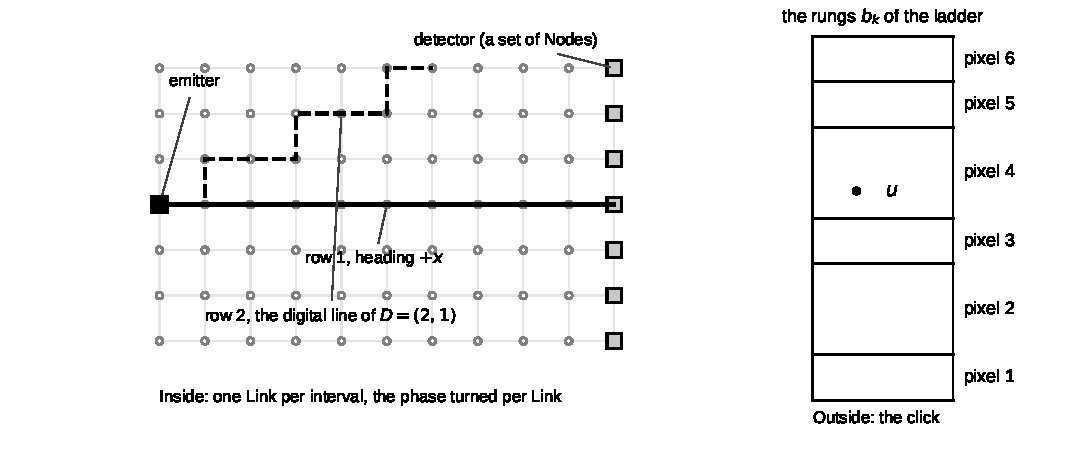
\includegraphics[width=0.96\linewidth]{figures/mechanism.pdf}\caption{\label{fig:mechanism}The mechanism, drawn from the definitions and no run. Inside (left): a GameBoard of Nodes joined by Links; an emitter puts one record of two rows on the board, each row on the digital line of its direction at one Link per interval, its phase turned per Link, nothing kept at a Node; a detector is a set of Nodes. Outside (right): the click, one comparison of the record's birth phase $u$ against the rungs of its ladder (Eq.~\eqref{eq:rung}); the cell $u$ falls in is the outcome, and the record is deleted. Nothing else is read.}\end{figure}

\begin{figure}[!tb]\centering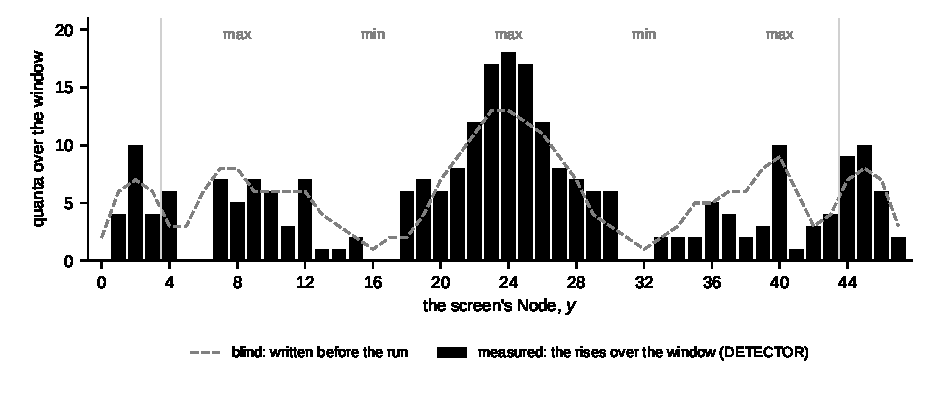
\includegraphics[width=0.48\linewidth]{figures/two_slits.pdf}\hfill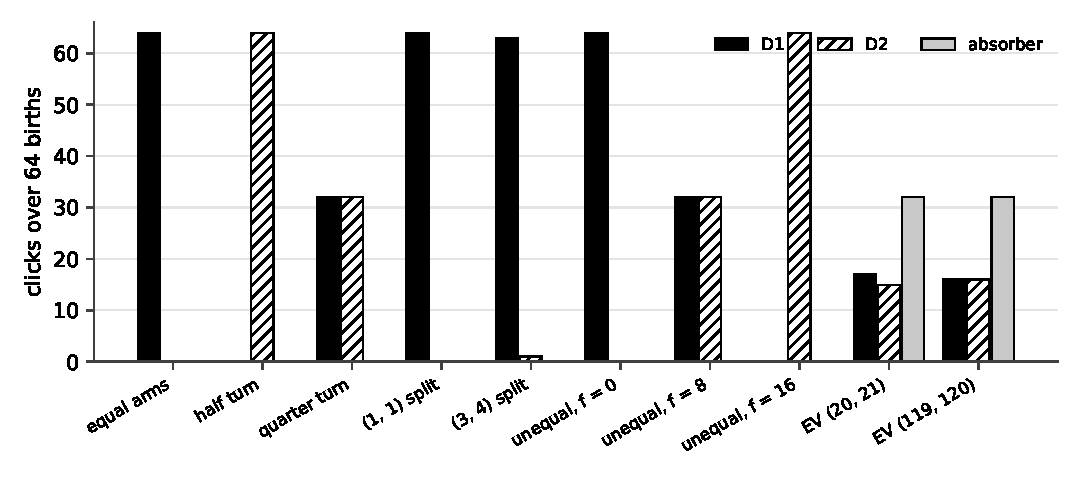
\includegraphics[width=0.48\linewidth]{figures/mach_zehnder.pdf}\caption{\label{fig:interference}Interference read at a detector, from the runs of series L at $\Nphi = 64$ (the figures' runs, Appendix~\ref{app:reproduction}). Left, the two-slit world \texttt{slits\_huygens}: above, the record's weight per pixel of the screen, a number of the board (GAMEBOARD, a diagnostic); below, the clicks over $64$ births (DETECTOR) and the histogram conditioned on the screen, bright where the two rows' ages differ by whole turns. Right, the Mach-Zehnder worlds: the clicks over $64$ births at the two ports and the absorber (DETECTOR), equal arms $64/0$, a half turn $0/64$, a quarter turn $32/32$, the $(1, 1)$ and $(3, 4)$ splits, the unequal arms and the two Elitzur-Vaidman worlds (Table~\ref{tab:nature}, row 2b; Appendix~\ref{app:reproduction}).}\end{figure}

\begin{figure}[!tb]\centering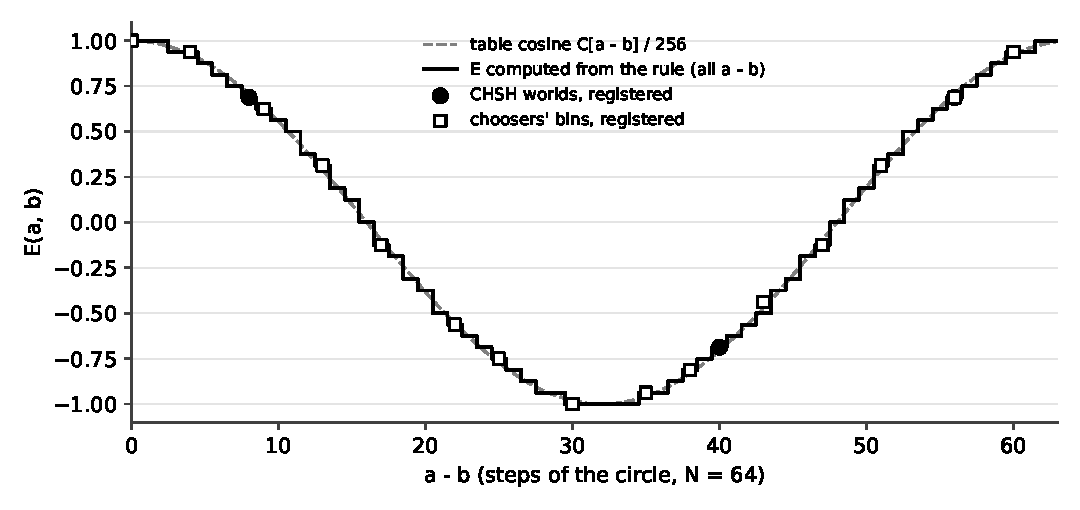
\includegraphics[width=0.8\linewidth]{figures/pair_64.pdf}\caption{\label{fig:pair}The pair at $\Nphi = 64$: $E(a, b)$ computed from the rule at every setting difference $a - b$ (the counts of Theorem~\ref{th:marginals} with the repository's tables, a computation \cite{checks}), the tables' cosine $C[a - b]/256$ dashed, and after a detector the registered CHSH worlds (circles) and the choosers' bins (squares) of series L (DETECTOR).}\end{figure}

\begin{figure}[!tb]
\begin{minipage}[c]{0.5\linewidth}\centering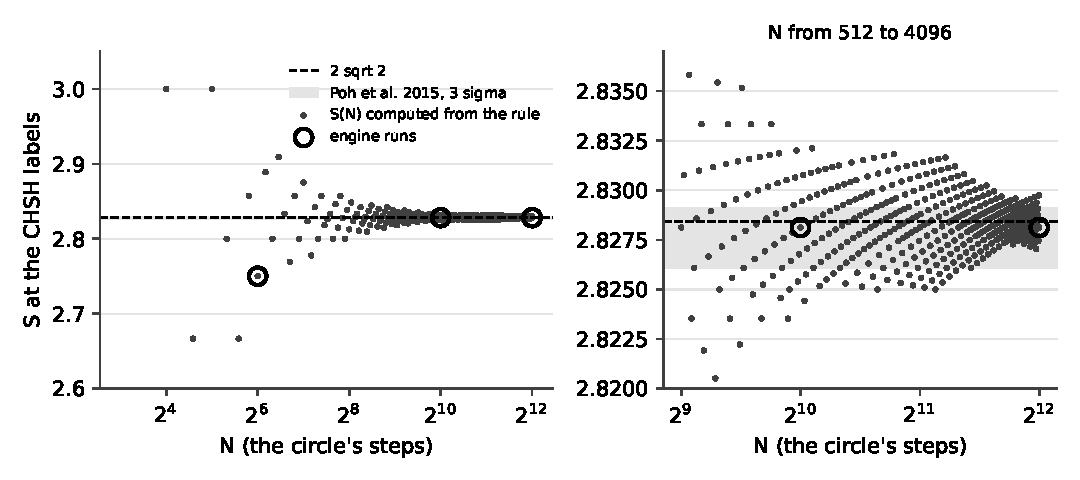
\includegraphics[width=\linewidth]{figures/s_of_n.pdf}\end{minipage}\hfill
\begin{minipage}[c]{0.47\linewidth}\caption{\label{fig:sofn}$S(\Nphi)$ at the CHSH labels. The curve is the closed form $S(\Nphi) = 8(c_1 + c_1')/\Nphi - 4$ computed from the rule at every multiple of $8$ with the tables at $N_t = 256$, a computation \cite{checks}; the circles are detector readings (DETECTOR) at $\Nphi = 64$, $512$, $1024$, $2048$, $4096$, $8192$ and $16384$ (series L, L6 and the register's block of the derivation's 24.4, the last three \cite[at b34fe114]{register}); the inset marks the plateau $181/64$ from $512$ through $8192$ and its end $5793/2048$ at $16384$; the dashed line is $2\sqrt2$.}\end{minipage}
\end{figure}
